\section*{Supplementary Material}

\begin{center}
	\vspace*{1cm} % Force vertical space below header
	\textbf{\LARGE 		Omnisoot: an object oriented package for process design of gas phase synthesis of Carbon black} 
\end{center}

\begin{center}
	Mohammad Adib$^{1,*}$, Sina Kazemi$^1$, M. Reza Kholgy$^{1,*}$ \\
	{\small *Corresponding author} \\
	$^1$ Department of Mechanical and Aerospace Engineering, Carleton University, 1125 Colonel By Dr, Ottawa, ON K1S 5B6, Canada
\end{center}

\beginsupplement


\section{The Effect of formation and sensible energy of soot}

\begin{figure}[H]
	\centering
	\begin{subfigure}[t]{0.43\textwidth}
		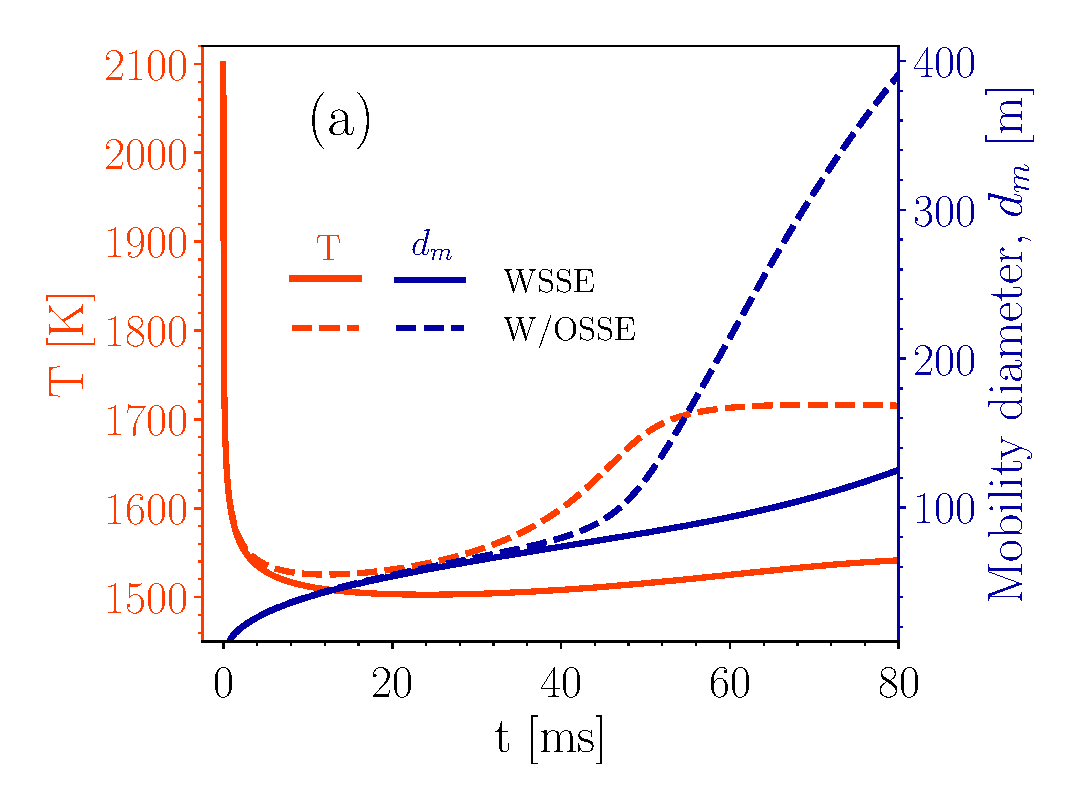
\includegraphics[width=1\textwidth]{Figures/Theory/sse_temp_dm.pdf}
	\end{subfigure}
	\begin{subfigure}[t]{0.4\textwidth}
		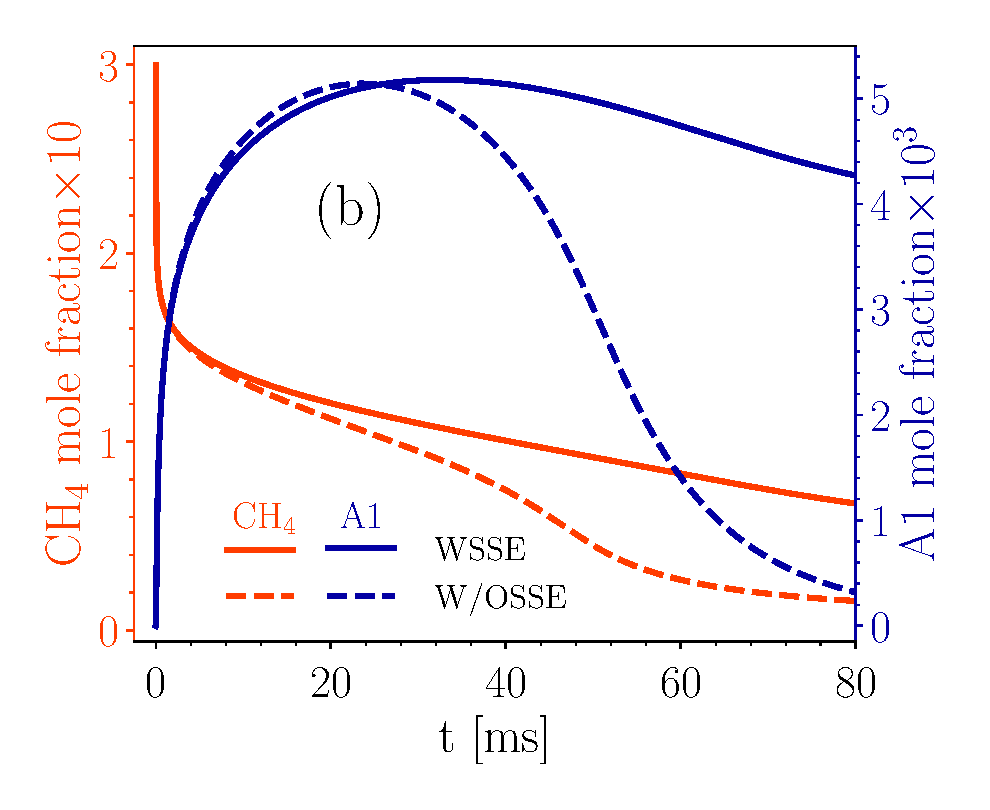
\includegraphics[width=1\textwidth]{Figures/Theory/sse_gasresid.pdf}
	\end{subfigure}
	\caption{The comparison of temperature and soot mobility diameter, $d_m$ (a) and the mole fraction of methane, $\mathrm{CH_4}$, and benzene, A1, in the simulation of the pyrolysis of 30\%~$\mathrm{CH_4}$-Ar when soot sensible energy is considered (labeled as ``WSSE") and neglected (labeled as ``W/OSSE"). The CVR was used along with Caltech mechanism~\citep{blanquart2009chemical}, Reactive Dimerization and MPBM.}
	\label{fig:sseeffect}
\end{figure}

\section{Diffusion of soot particles}
\label{sec:diffcoef}
% [Might be removed to the supplumenatary material for the paper]
The diffusion coefficient of soot particle, $D^i$, is calculated as:

\begin{equation}
	D^i = \frac{k_B T}{f^i}
	\label{eqn:diff},
\end{equation}
\noindent where $f^i$ is the friction factor of particles in gas and is calculated as:

\begin{equation}
	f^i = \frac{3\pi\mu d^i_m}{C^i(d^i_m)},
	\label{eqn:fraction}
\end{equation}

\noindent where ${C^i}$ is the Cunningham correction factor that accounts for non-continuum effects in the transition and free-molecular regimes. ${C^i}$ is calculated for a given diameter, $d$, as: 
\begin{equation}
	C^i(d) = 1+\frac{2\lambda}{d}
	\left(
	1.21+0.4\cdot\mathrm{exp}(\frac{-0.78d}{\lambda})
	\right)
	\label{eqn:cun},
\end{equation}
\noindent  where $\lambda$ is the mean free path of gas given as:
\begin{equation}
	\lambda = \frac{\mu}{\rho}\sqrt{\frac{\pi \cdot W_{gas}}{2k_B \cdot Av \cdot T}}
	\label{eqn:lambda}.
\end{equation}
Note that $\lambda$ is a property of the gas mixture that does not depend on particle mass and morphology. 

\section{Sectional Population Balance Model}
\label{sec:sectextra}

\subsection{Coagulation Source Term}
\label{sec:sectcoagsource}
Coagulation redistributes the total number of agglomerates and primary particles as well as hydrogen atoms among the sections. The partial coagulation source terms for ${N^i_{agg}}$, ${N^i_{pri}}$ and ${H^i_{tot}}$ can be calculated as:

\begin{equation}
	\left(S^i_{N_{agg}}\right)_{coag}
	=
	\sum_{k=1}^{n_{sec}}\sum_{j=k}^{n_{sec}}
	\left(
	1-\frac{\delta_{jk}}{2}
	\right)
	\eta_{ijk}\zeta^{jk}\beta^{jk}N^j_{agg}N^k_{agg}
	-
	N^i_{agg}
	\sum_{m=1}^{n_{sec}}\zeta^{im}\beta^{im}N^m_{agg},
	\label{eqn:IcoagNaggsect}
\end{equation}

\begin{equation}
	\left(S^i_{N_{pri}}\right)_{coag}
	=
	\sum_{k=1}^{n_{sec}}\sum_{j=k}^{n_{sec}}
	\left(
	1-\frac{\delta_{jk}}{2}
	\right)
	\eta_{p,ijk}\eta_{ijk}\zeta^{jk}\beta^{jk}N^j_{agg}N^k_{agg}
	-
	N^i_{pri}
	\sum_{m=1}^{n_{sec}}\zeta^{im}\beta^{im}N^m_{agg},
	\label{eqn:IcoagNprisect}
\end{equation}

\begin{equation}
	\left(S^i_{H_{tot}}\right)_{coag}
	=
	\sum_{k=1}^{n_{sec}}\sum_{j=k}^{n_{sec}}
	\left(
	1-\frac{\delta_{jk}}{2}
	\right)
	\eta_{h,ijk}\eta_{ijk}\zeta^{jk}\beta^{jk}N^j_{agg}N^k_{agg}
	-
	H^i_{tot}
	\sum_{m=1}^{n_{sec}}\zeta^{im}\beta^{im}N^m_{agg}.
	\label{eqn:IcoagHtotsect}
\end{equation}
\noindent where ${\delta_{jk}}$ is the Kronecker delta defined as:

\begin{equation}
	\delta_{jk}=
	\left\{
	\begin{array}{lr}
		1, & \text{if } j = k\\
		0. & \text{if } j \neq k
	\end{array}
	\right.
	\label{eqn:deltakronecker}
\end{equation}

The collision frequency between sections $j$ and $k$ ($\beta^{jk}$) can be obtained from the harmonic mean of the values in the continuum ($\beta_{cont}^{jk}$) and free molecular ($\beta_{fm}^{jk}$) regimes as:

\begin{equation}
	\beta^{jk} = 				       \frac{\beta^{jk}_{fm}\cdot\beta^{jk}_{cont}}{\beta^{jk}_{fm}
		+\beta^{jk}_{cont}}
	\label{eqn:betahmsect},
\end{equation}

\begin{equation}
	\beta^{jk}_{fm} =
	\sqrt{
		\frac{\pi k_B T}{2}
		\left(
		\frac{1}{m^j_{agg}}+
		\frac{1}{m^k_{agg}}
		\right)
	} 
	\left(
	d^j_c+d^k_c
	\right)^2
	\label{eqn:betafmsect},
\end{equation}
\begin{equation}
	\beta^{ij}_{cont} = \frac{2k_BT}{3\mu}
	\left(
	\frac{C^j}{d^j_m}+
	\frac{C^k}{d^k_m}
	\right)
	\left(
	d^j_c+d^k_c
	\right)^2
	\label{eqn:betacontsect}.
\end{equation}

The collision frequency can also be determined from the Fuchs interpolation as:

\begin{equation}
	\beta^{jk}=
	\beta^{ij}_{cont}
	\left[
	\frac{d^j_c+d^k_c}{d^j_c+d^k_c+2+\delta^{jk}_r}+
	\frac{8\left(D^j+D^k\right)}
	{\bar{c}^{jk}_r\left(d^j_c+d^k_c\right)}
	\right]^{-1},
	\label{eqn:betafuchssect}
\end{equation}
\noindent where ${\delta^{jk}_r}$ and ${\bar{c}^{jk}_r}$ are the mean square root of mean distance and velocity of particles, respectively, and they are obtained as:

\begin{equation}
	\delta^{jk}_r=
	\sqrt{
		{\delta^j_a}^2+{\delta^k_a}^2
	}
	\label{eqn:sqrtmeandist},
\end{equation}

\begin{equation}
	\bar{c}^{jk}_r=
	\sqrt{
		{c^j}^2+{c^k}^2
	}
	\label{eqn:sqrtmeanvel}.
\end{equation}

The mean velocity, ${c^i}$, and mean stop distance of particles, ${\lambda^i_a}$, can be calculated as:

\begin{equation}
	c^i = \sqrt{\frac{8k_B T}{\pi m^i_{agg}}},
	\label{eqn:meanvel}
\end{equation}

\begin{equation}
	\delta^i_a=\frac{1}{d^i_c\lambda^i_a}
	\left[
	\left(
	d^i_c+\lambda^i_a
	\right)^3
	-\left(
	{d^i_c}^2+{\lambda^i_a}^2
	\right)^{3 / 2}
	\right]
	-d^i_{c},
	\label{eqn:meandist}
\end{equation}
\noindent $\lambda^i_a $is the agglomerate stopping distance defined as:
\begin{equation}
	\lambda^i_a = \frac{8D^i}{\pi c^i}
	\label{eqn:stopdist}.
\end{equation}




In Equation~\eqref{eqn:IcoagNaggsect}, $\mathrm{\eta_{ijk}}$ assigns newly formed agglomerates to the two consecutive sections in order to conserve mass during coagulation~\citep{park2005aerosol}.

\begin{equation}
	\eta_{ijk}=
	\left\{
	\begin{aligned}
		&\frac{C^{i+1}_{agg}-C^{jk}_{agg}}{C^{i+1}_{agg}-C^i_{agg}},
		&&
		\text{if } C^i_{agg} \le C^{jk}_{agg} < C^{i+1}_{agg}
		\\
		&\frac{C^{i}_{agg}-C^{jk}_{agg}}{C^{i}_{agg}-C^{i-1}_{agg}}, 
		&&
		\text{if } C^{i-1}_{agg} \le C^{jk}_{agg} < C^{i}_{agg}
		\\
		&0,
		&&\text{else}
	\end{aligned}
	\right.
	\label{eqn:etacoag}
\end{equation}
\noindent where ${C^{jk}_{agg}=C^{j}_{agg}+C^{k}_{agg}}$. Similarly, $\eta_{p,ijk}$ in Equation~\eqref{eqn:IcoagNprisect} and $\eta_{h,ijk}$ in Equation~\eqref{eqn:IcoagHtotsect} adjust the number of primary particles and hydrogen atoms added to consecutive sections based on their mass, respectively.

\begin{equation}
	\eta_{p,ijk}=
	\frac{C^i_{agg}}{C^{jk}_{agg}}
	\left(
	n^j_p + n^k_p
	\right),
	\label{eqn:etapcoag}
\end{equation}

\begin{equation}
	\eta_{h,ijk}=
	\frac{C^i_{agg}}{C^{jk}_{agg}}
	\left(
	H^j_{agg} + H^k_{agg}
	\right).
	\label{eqn:etahcoag}
\end{equation}


In Equation~\eqref{eqn:IcoagNaggsect}, $\zeta^{jk}$ is the coagulation efficiency of soot particles in sections $j$ and $k$. A value of $\zeta^{jk} = 1$ indicates that every collision between two soot particles successfully results in the formation of a new agglomerate. However, numerical models~\citep{narsimhan1985brownian} and experimental evidence~\citep{d2005surface} have shown that coagulation efficiency drastically decreases for particles smaller than 10~nm in the free-molecular regime ($\mathrm{Kn}\gg10$), due to their high kinetic energy exceeding the magnitude of attractive forces~\citep{wang1991filtration}. The coagulation efficiency between two colliding particles can be described by~\citep{narsimhan1985brownian}:


\begin{equation}
	\zeta^{ij} = 1 - 
	\left(1 + \frac{\Phi^{ij}_0}{k_BT} \right)
	\mathrm{exp}\left(-\frac{\Phi^{ij}_0}{k_BT}\right),
	\label{eqn:coageff}
\end{equation}

\noindent where $\Phi_0$ is the potential well depth, i.e., the minimum interaction energy between two colliding particles. \citet{hou2020coagulation} calculated $\Phi_0$ for soot particles ranging from 1 to 15 nm by considering the attractive and repulsive interactions between constituent carbon and hydrogen atoms, and proposed an equation based on the reduced diameter, $d^{jk}_r$, of colliding particles as:

\begin{equation}
	\Phi^{ij}_0 = -6.6891\times10^{-23} (d^{jk}_r)^3 + 1.1244\times10^{-21} (d^{jk}_r)^2 + 1.1394\times10^{-20} d^{jk}_r - 5.5373\times10^{-21},
	\label{eqn:coageffphi}
\end{equation}

\begin{equation}
	d^{jk}_r = \frac{d^i_c\cdot d^j_c}{d^i_c+d^j_c}.
	\label{eqn:coageffredcueddia}
\end{equation}

Equation~\eqref{eqn:coageffphi} is valid for $d^{jk}_r$ between 1 and 7~nm, and $\zeta^{ij}$ is assumed as unity for particles with a reduced diameter larger than 7~nm.


\subsection{Other Source terms}
\label{sec:sectothersource}

Inception introduces equal number of agglomerates and primary particles to the first section.

\begin{equation}
	\begin{aligned}
		\left(S^i_{N_{agg}}\right)_{inc} =
		&\frac{1}{Av}\frac{I_{N, inc}}{C^i_{agg}}, && i=1.
	\end{aligned}
	\label{eqn:S_Nagg_incsect}
\end{equation}

\begin{equation}
	\begin{aligned}
		\left(S^i_{N_{pri}}\right)_{inc} =
		&\frac{1}{Av}\frac{I_{N, inc}}{C^i_{agg}}, && i=1.
	\end{aligned}
	\label{eqn:S_Npri_incsect}
\end{equation}

\begin{equation}
	\begin{aligned}
		\left(S^i_{H_{tot}}\right)_{inc} =
		&I_{H, inc}, && i=1.
	\end{aligned}
	\label{eqn:S_Htot_incsect}
\end{equation}
Surface growth and PAH adsorption increase both the carbon mass and hydrogen content of agglomerates, transferring them to higher sections. The rate at which agglomerates are removed from the original section and added to the target section is calculated to ensure mass conservation. Specifically, it is determined by dividing the mass growth rate by the difference in mass between adjacent sections as:


\begin{equation}
	\left(S^i_{N_{agg}}\right)_{haca, ads}=
	\frac{1}{Av}
	\left\{
	\begin{aligned}
		&-\frac{I^i_{C_{tot},haca}+I^i_{C_{tot},ads}}{C^{i+1}_{agg}-C^{i}_{agg}},
		&&
		\text{if } i = 1
		\\
		&\frac{I^{i-1}_{C_{tot},haca}+I^{i-1}_{C_{tot},haca}}{C^{i}_{agg}-C^{i-1}_{agg}}
		-\frac{I^{i}_{C_{tot},haca}+I^{i}_{C_{tot},ads}}{C^{i+1}_{agg}-C^{i}_{agg}},
		&&
		\text{if } 1 < i < n_{sec}
		\\
		&\frac{I^{i-1}_{C_{tot},haca}+I^{i-1}_{C_{tot},ads}}{C^{i}_{agg}-C^{i-1}_{agg}}.
		&&\text{if } i=n_{sec}
	\end{aligned}
	\right.
	\label{eqn:S_Nagg_gradssect}
\end{equation}

As agglomerates move up/down through sections, they carry the number of primary particles as well as hydrogen atoms, so the transfer rate of agglomerates is multiplied by ${n^i_p}$ and ${H^i_{agg}}$, respectively. 

\begin{equation}
	\left(S^i_{N_{pri}}\right)_{haca, ads}=
	\frac{1}{Av}
	\left\{
	\begin{aligned}
		&-\frac{I^i_{C_{tot},haca}+I^i_{C_{tot},ads}}{C^{i+1}_{agg}-C^{i}_{agg}},
		&&
		\text{if } i = 1
		\\
		&\frac{I^{i-1}_{C_{tot},haca}+I^{i-1}_{C_{tot},ads}}{C^{i}_{agg}-C^{i-1}_{agg}}n^{i-1}_p
		-\frac{I^{i}_{C_{tot},haca}+I^{i}_{C_{tot},ads}}{C^{i+1}_{agg}-C^{i}_{agg}}n^{i}_p,
		&&
		\text{if } 1 < i < n_{sec}
		\\
		&\frac{I^{i-1}_{C_{tot},haca}+I^{i-1}_{C_{tot},ads}}{C^{i}_{agg}-C^{i-1}_{agg}}n^{i-1}_p,
		&&\text{if } i=n_{sec}
	\end{aligned}
	\right.
	\label{eqn:S_Npri_gradssect}
\end{equation}

\begin{equation}
	\left(S^i_{H_{tot}}\right)_{haca, ads}=
	\frac{1}{Av}
	\left\{
	\begin{aligned}
		&-\frac{I^i_{C_{tot},haca}+I^i_{C_{tot},ads}}{C^{i+1}_{agg}-C^{i}_{agg}}H^{i}_{agg} 
		+ I^{i}_{H_{tot}, haca} + I^{i}_{H_{tot}, ads},
		&&
		\text{if } i = 1
		\\
		&\frac{I^{i-1}_{C_{tot},haca}+I^{i-1}_{C_{tot},ads}}{C^{i}_{agg}-C^{i-1}_{agg}}H^{i-1}_{agg}
		-\frac{I^{i}_{C_{tot},haca}+I^{i}_{C_{tot},ads}}{C^{i+1}_{agg}-C^{i}_{agg}}H^{i}_{agg}
		+ I^{i}_{H_{tot}, haca} + I^{i}_{H_{tot}, ads},
		&&
		\text{if } 1 < i < n_{sec}
		\\
		&\frac{I^{i-1}_{C_{tot},haca}+I^{i-1}_{C_{tot},ads}}{C^{i}_{agg}-C^{i-1}_{agg}}H^{i-1}_{agg}
		+ I^{i}_{H_{tot}, haca} + I^{i}_{H_{tot}, ads}.
		&&\text{if } i=n_{sec}
	\end{aligned}
	\right.
	\label{eqn:S_Htot_gradssect}
\end{equation}

Similarly, the agglomerates lose carbon mass by oxidation, and descend to the lower sections carrying primary particle and hydrogen.

\begin{equation}
	\left(S^i_{N_{agg}}\right)_{ox}=
	\frac{1}{Av}
	\left\{
	\begin{aligned}
		&\frac{I^{i+1}_{C_{tot},ox}}{C^{i+1}_{agg}-C^{i}_{agg}}
		-
		\frac{I^{i}_{C_{tot},ox}}{C^{i}_{agg}},
		&&
		\text{if } i = 1
		\\
		&\frac{I^{i+1}_{C_{tot},ox}}{C^{i+1}_{agg}-C^{i}_{agg}}
		-
		\frac{I^{i}_{C_{tot},ox}}{C^{i}_{agg}-C^{i-1}_{agg}},
		&&
		\text{if } 1 < i < n_{sec}
		\\
		&
		-
		\frac{I^{i}_{C_{tot},ox}}{C^{i}_{agg}-C^{i-1}_{agg}},
		&&\text{if } i=n_{sec}
	\end{aligned}
	\right.
	\label{eqn:S_Nagg_oxsect}
\end{equation}

\begin{equation}
	\left(S^i_{N_{pri}}\right)_{ox}=
	\frac{1}{Av}
	\left\{
	\begin{aligned}
		&\frac{I^{i+1}_{C_{tot},ox}}{C^{i+1}_{agg}-C^{i}_{agg}}n^{i+1}_p
		-
		\frac{I^{i}_{C_{tot},ox}}{C^{i}_{agg}},
		&&
		\text{if } i = 1
		\\
		&\frac{I^{i+1}_{C_{tot},ox}}{C^{i+1}_{agg}-C^{i}_{agg}}n^{i+1}_p
		-
		\frac{I^{i}_{C_{tot},ox}}{C^{i}_{agg}-C^{i-1}_{agg}}n^{i}_p,
		&&
		\text{if } 1 < i < n_{sec}
		\\
		&
		-
		\frac{I^{i}_{C_{tot},ox}}{C^{i}_{agg}-C^{i-1}_{agg}}n^{i}_p,
		&&\text{if } i=n_{sec}
	\end{aligned}
	\right.
	\label{eqn:S_Npri_oxsect}
\end{equation}

\begin{equation}
	\left(S^i_{H_{tot}}\right)_{ox}=
	\frac{1}{Av}
	\left\{
	\begin{aligned}
		&\frac{I^{i+1}_{C_{tot},ox}}{C^{i+1}_{agg}-C^{i}_{agg}}H^{i+1}_{agg}
		-
		\frac{I^{i}_{C_{tot},ox}}{C^{i}_{agg}}H^{i}_{agg}
		+ I^{i}_{H_{tot}, ox},
		&&
		\text{if } i = 1
		\\
		&\frac{I^{i+1}_{C_{tot},ox}}{C^{i+1}_{agg}-C^{i}_{agg}}H^{i+1}_{agg}
		-
		\frac{I^{i}_{C_{tot},ox}}{C^{i}_{agg}-C^{i-1}_{agg}}H^{i}_{agg}
		+ I^{i}_{H_{tot}, ox},
		&&
		\text{if } 1 < i < n_{sec}
		\\
		&
		-
		\frac{I^{i}_{C_{tot},ox}}{C^{i}_{agg}-C^{i-1}_{agg}}H^{i}_{agg}
		+ I^{i}_{H_{tot}, ox}.
		&&\text{if } i=n_{sec}
	\end{aligned}
	\right.
	\label{eqn:S_Htot_oxsect}
\end{equation}



\section{PAH growth models}

\subsection{Irreversible Dimerization}
\label{sec:irrevdim}

The Irreversible Dimerization is based on the collision of a pair of PAH molecules forming a dimer. The sequential growth continues leading formation of trimers and tetramers until the PAH cluster mass reaches a threshold that can be considered a solid particle. For practical purposes, a dimer is usually considered as an incipient particle that grows by surface growth and coagulation. A single-step collision of two similar PAHs forms a new dimer as:

\reaction[react:irrevdiminc]{
	$\mathrm{PAH}_j$ + $\mathrm{PAH}_j$ ->[$k_{f,dim_j}$] $\mathrm{Dimer}_j$
}
Similarly, the adsorption of each PAH molecule on soot particles is described by the irreversible collision of soot and $\mathrm{PAH}_j$ as:
\reaction[react:irrevdimads]{
	$\mathrm{PAH}_j$ + Soot ->[$k_{f,ads_j}$] Soot-$\mathrm{PAH}_j$
}
The forward rate of dimerization, ${k_{f,dim_j}}$, and adsorption, $k_{f,ads_j}$, in Reactions~\eqref{react:irrevdiminc} and \eqref{react:irrevdimads} are calculated as:

\begin{equation}
	k_{f,dim_j}=
	\gamma_{inc}\cdot\beta_{jj,PAH}\cdot Av
	\label{eqn:kfdim},
\end{equation}

\begin{equation}
	k^i_{f,ads_j}=
	\gamma_{ads_j}\cdot\beta^i_{j,ads}\cdot Av
	\label{eqn:kfads},
\end{equation}

\noindent where $\beta_{jk,\mathrm{PAH}}$ and $\beta^i_{j,\mathrm{ads}}$ are computed using Equations~\eqref{eqn:betadim} and~\eqref{eqn:betahmads}, respectively, and $\gamma_{\mathrm{inc}}$ and $\gamma_{\mathrm{ads}}$ are the collision efficiencies for dimerization and adsorption, respectively. Their values range from $\mathrm{10^{-7}}$ to 1 and are typically chosen to match the predicted soot properties with experimental data. The dimerization rate of $\mathrm{PAH}_j$ is then calculated as:

\begin{equation}
	w_{dim_j} = \eta_{inc} k_{f,dim_{j}} [\mathrm{PAH}_j] [\mathrm{PAH}_j].
	\label{eqn:irrevdim_wdim}
\end{equation}

The partial source terms of inception are calculated as:

\begin{equation}
	I_{N,inc} =\frac{1}{\rho} \sum_{j=1}^{n_{PAH}} 2w_{dim_j} n_{PAH_j,C},
	\label{eqn:INinc}
\end{equation}
\begin{equation}
	I_{C_{tot},inc} = \frac{1}{\rho}\sum_{j=1}^{n_{PAH}} 2w_{dim_j} n_{PAH_j,C}.
	\label{eqn:ICtotinc}
\end{equation}
\begin{equation}
	I_{H_{tot},inc} =\frac{1}{\rho} \sum_{j=1}^{n_{PAH}} 2w_{dim_j} n_{PAH_j,H}.
	\label{eqn:IHtotinc}
\end{equation}
The rate of PAH adsorption for each section is obtained as:
\begin{equation}
	w^i_{ads_j} = \eta_{ads} k^i_{f,ads_{j}} [\mathrm{soot}^i] [\mathrm{PAH}_j].
	\label{eqn:adsrate_irrevdim}
\end{equation}

The contribution of PAH adsorption to the source terms are expressed as:

\begin{equation}
	I^i_{C_{tot},ads} = \frac{1}{\rho}\sum_{j=1}^{n_{PAH_j}} w^i_{ads_j} n_{PAH_j,C},
	\label{eqn:ICtotads}
\end{equation}
\begin{equation}
	I^i_{H_{tot},ads} =\frac{1}{\rho} \sum_{j=1}^{n_{PAH_j}} w^i_{ads_j} (n_{PAH_j,H}-2).
	\label{eqn:IHtotads}
\end{equation}

Note that PAH adsorption is a mass growth phenomenon that only changes $C_{tot}$ and $H_{tot}$ but does not affect number of $N_{agg}$ and $N_{pri}$. Each PAH molecule loses one H atom becoming a radical that forms bonds with a dehydrogenated site on soot surface, so two H atoms are released during adsorption that is taken into account in Equation~\eqref{eqn:IHtotads}.

The formation of a dimer consumes two PAH molecules, and during adsorption one PAH molecule is removed from the gas mixture, so the total rate of removal of $\mathrm{PAH}_j$ by Irreversible Dimerization is obtained as:

\begin{equation}
	\left(
	\frac{d\left[{\mathrm{PAH}_j}\right]}{dt}
	\right)_{inc}
	= 
	-2w_{dim_j},
	\label{eqn:PAHscrub_irrevdim_inc}
\end{equation}

\begin{equation}
	\left(
	\frac{d\left[{\mathrm{PAH}_j}\right]}{dt}
	\right)_{inc}
	= 
	-\sum_{i=1}^{n_{sec}}w^i_{ads_j}.
	\label{eqn:PAHscrub_irrevdim_ads}
\end{equation}

Moreover, one $\mathrm{H_2}$ is released to the gas mixture as a result of the adsorption process.
\begin{equation}
	\left(
	\frac{d\left[{\mathrm{H_2}}\right]}{dt}
	\right)_{ads}
	= 
	\sum_{i=1}^{n_{sec}}w^i_{ads_j}
	\label{eqn:H2scrub_irrevdim}.
\end{equation}


\subsection{Reactive Dimerization}
\label{sec:reacvdim}

This model was built on Irreversible Dimerization with a main difference: The first step of dimerization and adsorption is reversible forming physically bonded dimers followed by a irreversible carbonization that leads to chemical bond formation in dimers \citep{kholghy2018reactive}. This approach allows the formation of homo- and hetero-dimers. The dimerization of $\mathrm{PAH}_j$ and $\mathrm{PAH}_k$ is described as:
\reaction[reac:phydim_reacdim]{
	PAH_j + PAH_k <-->[$k_{f,dim_{jk}}$][$k_{r,dim_{jk}}$] Dimer^*_{$ij$}
}
\reaction[reac:chemdim_reacdim]{
	Dimer^*_{$jk$} ->[$k_{reac}$] Dimer_{$jk$}
}
\noindent where $\mathrm{Dimer^*}_{jk}$ and $\mathrm{Dimer}_{jk}$ are physically and chemically bonded dimers, respectively, from $\mathrm{PAH}_j$ and $\mathrm{PAH}_k$. The forward rate of physical dimerization, ${k_{f,dim_{jk}}}$, is calculated as:

\begin{equation}
	k_{f,dim_{jk}}=
	p^{''}\cdot\beta_{jk,PAH}\cdot Av
	\label{eqn:kfphydim_reacdim},
\end{equation}

\noindent where $\beta_{jk,\mathrm{PAH}}$ is calculated using Equation~\eqref{eqn:betadim}, and $p^{\prime\prime} = 0.1$ accounts for the probability of PAH–PAH collisions occurring in the "FACE" configuration that result in successful van der Waals (vdW) bond formation~\citep{miller1984intermolecular}. The reverse rate of physical dimerization, $k_{r,\mathrm{dim}_{jk}}$, is obtained from the dimerization equilibrium constant~\citep{miller1991kinetics} as:


\begin{equation}
	k_{r,dim_{jk}} = \frac{k_{f,dim_{jk}}}{K_{eq}} 
	\label{eqn:krphydim_reacdim},
\end{equation}

\begin{equation}
	\mathrm{log}_{10}K_{eq}=
	a\frac{\epsilon_{jk}}{RT}+b
	\label{eqn:keq_reacdim},
\end{equation}

\begin{equation}
	\epsilon_{jk} = cW_{jk} -d
	\label{eqn:epsilon_reacdim},
\end{equation}

\begin{equation}
	W_{jk} = \frac{W_j\cdot W_k}{W_j+W_k}
	\label{eqn:Wjk_reacdim},
\end{equation}
\noindent where $a=0.115$ (obtained from pyrere dimerization data~\citep{sabbah2010exploring}) and $b=1.8$~\citep{kholghy2018reactive}, $c=933420$~J/kg, and $d=34053$~J/mol~\cite{kholghy2018reactive}. 

The rate constant of chemical bond formation, $k_{reac}$, is defined in the Arrhenius form~\cite{naseri2022simulating} as
\begin{equation}
	k_{reac} = 5\times10^6\cdot e^{(-96232/RT)}
	\label{eqn:kc_reacdim}.
\end{equation}

Assuming a steady state condition for physical dimers, i.e., $\mathrm{\partial [Dimer^*_{jk}]/\partial t=0}$, the rate of formation of chemically-bonded dimers can be obtained as:

\begin{equation}
	\omega_{dim_{jk}} = k_{reac}\frac{k_{f,dim_{jk}}[\mathrm{PAH}_j][\mathrm{PAH}_k]}
	{k_{r,dim_{jk}}+k_{reac}}
	\label{eqn:chemdimer_reacdim}.
\end{equation}

The contribution of dimer formation to the partial source terms is evaluated by looping over all combinations of PAH precursors as:


\begin{equation}
	I_{N,{inc}} = 
	\frac{1}{\rho}
	\sum_{j=1}^{n_{PAH}} \sum_{k=j}^{n_{PAH}}  \omega_{dim_{kj}} 
	\left(
	n_{PAH_j,C}+n_{PAH_k,C}
	\right),
	\label{eqn:IN_inc}
\end{equation}

\begin{equation}
	I_{C_{tot},{inc}} = 
	\frac{1}{\rho}
	\sum_{j=1}^{n_{PAH}} \sum_{k=j}^{n_{PAH}}  \omega_{dim_{kj}} 
	\left(
	n_{PAH_j,C}+n_{PAH_k,C}
	\right),
	\label{eqn:ICtot_inc}
\end{equation}

\begin{equation}
	I_{H_{tot},{inc}} = 
	\frac{1}{\rho}
	\sum_{j=1}^{n_{PAH}} \sum_{k=j}^{n_{PAH}}  \omega_{dim_{kj}} 
	\left(
	n_{PAH_j,H}+n_{PAH_k,H}
	\right).
	\label{eqn:IHtot_inc}
\end{equation}

Similarly, PAH adsorption is described by a two-step process where the collision of $\mathrm{PAH}_j$ with soot agglomerates leads to a physically bonded Soot$-$$\mathrm{PAH}^*_j$ that is carbonized and forms a chemically bonded Soot$-$$\mathrm{PAH}_j$ on soot surface.

\reaction[reac:physootPAH_reacdim]{
	PAH_j + Soot <-->[$k_{f,ads_j}$][$k_{r,ads_j}$] Soot-PAH^*_j
}

\reaction[reac:chemsootPAH_reacdim]{
	Soot-PAH^*_j ->[$k_{c,ads}$] Soot-PAH_j
}

The forward and reverse rate of PAH-soot collision are calculated as:

\begin{equation}
	k^i_{f,ads_j}=\beta^i_{j,ads}\cdot Av,
	\label{eqn:kfads_reacdim}
\end{equation}

\begin{equation}
	k^i_{r,ads_j}=k^i_{f,ads_j}\cdot10^{-b}e^{-a\epsilon^i_{soot,j} \mathrm{ln}(10)/(RT)},
	\label{eqn:krads_reacdim}
\end{equation}

\begin{equation}
	\epsilon^i_{soot,j} = cW^i_{soot,j} - d,
	\label{eqn:epsilonads_reacdim}
\end{equation}

\noindent where $\beta^i_{j,ads}$ is calculated using Equation~\eqref{eqn:betahmads}. The values of $a$, $b$, $c$, and $d$ are the same as those explained in the inception part. Computing ${\epsilon^i_{soot,j}}$ also requires the equivalent soot molecular weight, ${W^i_{soot}}$, which is estimated from carbon mass of each agglomerate as:

\begin{equation}
	W^i_{soot}=\frac{C^i_{tot}W_{carbon}}{N^i_{agg}}.
\end{equation}

The rate constant of carbonization of Soot$-$$\mathrm{PAH}^*_j$ is defined as in an Arrhenius form similar to the inception formulation (Equation~\eqref{eqn:kc_reacdim}). The pre-exponential factor is adjusted by matching the numercial PSD~\citep{naseri2022simulating} with measurements in the ethylene pyrolysis in a flow reactor~\cite{araki2021effects}. 

\begin{equation}
	k_{c,ads} = 2\times10^{10}\cdot e^{(-96232/RT)}
	\label{eqn:kcads_reacdim}.
\end{equation}


The total adsorption rate can be calculated assuming a steady-state concentration for the physically adsorbed PAH on soot, i.e., $\partial$[Soot$-\mathrm{PAH}^*_j$]/$\partial t=0$, calculated in a similar way to the inception flux (Equation~\eqref{eqn:chemdimer_reacdim}) as:

\begin{equation}
	\omega^i_{ads_j} = k_{c,ads}\frac{k_{f,ads_j}[\mathrm{soot}^i][\mathrm{PAH}_j]}{k_{r,ads_j}+k_{c,ads_j}}
	\label{eqn:wads_reacdim},
\end{equation}

The contribution of PAH adsorption rate to the partial source terms can be expressed as:

\begin{equation}
	I^i_{C_{tot},ads} =
	\frac{1}{\rho}
	\sum_{i=1}^{n_{PAH}}
	\omega^i_{ads_j}
	n_{C,PAH_j}
	\label{eqn:ICtotads_reacdim},
\end{equation}

\begin{equation}
	I^i_{H_{tot},ads} =
	\frac{1}{\rho}
	\sum_{i=1}^{n_{PAH}}
	\omega^i_{ads_j}
	\left(n_{H,PAH_j}-2\right)
	\label{eqn:IHtotads_reacdim}.
\end{equation}

The rate of removal of PAH from the gas mixture due to inception and PAH adsorption is given as:

\begin{equation}
	\left(
	\frac{d\left[{\mathrm{PAH}_j}\right]}{dt}
	\right)_{inc}
	= 
	-\sum_{k=1}^{n_{PAH}}w_{dim_{jk}},
	\label{eqn:PAHscrub_inc_reacdim}
\end{equation}

\begin{equation}
	\left(
	\frac{d\left[{\mathrm{PAH}_j}\right]}{dt}
	\right)_{ads}
	= -\sum_{i=1}^{n_{sec}}w^i_{ads_j}.
	\label{eqn:PAHscrub_ads_reacdim}
\end{equation}

Additionally, during the PAH adsorption process one $\mathrm{H_2}$ is released to the gas mixture changing the concentration of $\mathrm{H_2}$ as:
\begin{equation}
	\left(
	\frac{d\left[{\mathrm{H_2}}\right]}{dt}
	\right)_{ads}
	= 
	\sum_{i=1}^{n_{sec}}w^i_{ads_j}
	\label{eqn:H2scrub_reacdim}.
\end{equation}

\subsection{Dimer Coalescence}
\label{sec:dimcoal}
The Dimer Coalescence model is a multi-step irreversible model proposed by \citet{blanquart2009joint} where self-collision of PAH molecules forms dimers, which are an intermediate state between gaseous PAH molecules and solid soot particles. The dimers can either form incipient soot particles through self-coalescence or adsorb on the surface of existing soot particles and contribute to their surface growth. The following equations describing the inception and surface growth in Dimer Coalescence adopted from the work of \citet{sun2021modelling}.

\reaction[reac:dim_dimcoal]{
	PAH_j + PAH_j ->[$k_{dim_{j}}$] Dimer_{j}
}
\reaction[reac:chemdim_reacdim]{
	Dimer_{j} + Dimer_{j} ->[$k_{inc_j}$] Tetramer_{j}
}
\reaction[reac:chemdim_reacdim]{
	Dimer_{j} + Soot ->[$k_{ads_j}$] Soot-PAH_{j}
}

The rate constant of dimerization, ${k_{dim_{j}}}$, and inception, ${k_{inc_{j}}}$, are calculated from the collision rate of PAHs as:

\begin{equation}
	k_{dim_{j}}=
	\gamma_{dim_j}\cdot\beta_{jj,PAH}\cdot Av
	\label{eqn:kdim_dimcoal},
\end{equation}

\begin{equation}
	k_{inc_{j}}=
	\beta_{jj,dimer}\cdot Av
	\label{eqn:kinc_dimcoal},
\end{equation}

\noindent where $\beta_{jj,PAH}$, $\beta_{jj,dimer}$ are both calculated using Equation~\eqref{eqn:betadim}. $\gamma_{dim_j}$ is the dimerization efficiency assumed to scale with the fourth power of the PAH molecular weight~\cite{blanquart2009analyzing} as:

\begin{equation}
	\gamma_{dim_j}=
	C_{N,j}\cdot W_{PAH_j}^4.
	\label{eqn:gamma_dimcoal}
\end{equation} 

\citet{blanquart2009joint} estimated the constant ${C_{N,j}}$ in Equation~\eqref{eqn:gamma_dimcoal} by comparing the profiles of several PAH species with the experimental measurements in a single premixed benzene flame~\citep{tregrossi1999combustion}, and provide ${C_{N,j}}$ values for various PAHs, which are listed in Table 1 in~\citep{blanquart2009analyzing}. The rate of dimer collision is expressed as:

\begin{equation}
	w_{dim_j} = \eta_{inc} k_{inc_{j}} [\mathrm{Dimer}_j] [\mathrm{Dimer}_j].
	\label{eqn:wdim_dimcoal}
\end{equation}


Similarly, the rate of adsorption of dimers on soot particles is obtained as:

\begin{equation}
	w^i_{ads_j} = \eta_{ads} k^i_{ads_{j}} [\mathrm{soot}^i] [\mathrm{Dimer}_j],
\end{equation}

\begin{equation}
	k^i_{ads_{j}}=
	\beta^i_{ads_j}\cdot Av.
	\label{eqn:kads_dimcoal}
\end{equation}

Assuming fast dimer consumption leads to the steady-state concentration of dimers, which can be determined by solving a quadratic equation~\citep{blanquart2009analyzing} as:
\begin{equation}
	a_{inc_j}[\mathrm{Dimer}_j]^2+b_{ads_j}[\mathrm{Dimer}_j]=\omega_{dim,j},
	\label{eqn:quad_dimcoal}
\end{equation}
\begin{equation}
	[\mathrm{Dimer}_j]=
	\left\{
	\begin{aligned}
		&\frac{-b_{ads_j}+\sqrt{\Delta_j}}{2a_{inc_j}},
		&&
		\text{if } \Delta_j \ge 0
		\\
		& 0 
		&&
		\text{if } \Delta_j < 0
	\end{aligned},
	\right.
	\label{eqn:dimer_dimcoal}
\end{equation}
\begin{equation}
	\Delta_j = b_{ads_j}^2+4a_{inc_j}\omega_{dim,j},
	\label{eqn:delta_dimcoal}
\end{equation}

\noindent where ${a_{inc_j} = k_{inc_{j}}}$ and ${b_{ads_j}}$ is calculated by summing the adsorption rate of dimers for all sections as:

\begin{equation}
	b_{ads_j} = \sum_{i=1}^{n_{sec}} k^i_{ads_{j}} [\mathrm{soot}^i]
\end{equation}

%\renewcommand{\arraystretch}{1.5}
%\begin{table}
%	\caption{The dimerization efficiency, $\mathrm{\gamma_{dim_j}}$, for different PAH in dimer coalescence model~\citep{blanquart2009analyzing}}
%	\label{tab:gammalist_dimcoal}
%	\centering
%	\begin{tabular}{l l l l}
	%		\hline
	%		Species name & Chemical formula & W~[kg/mol] & $\mathrm{\gamma_{dim_j}}$\\
	%		\hline
	%		Naphthalene & $\mathrm{C_{10}H_{8}}$ & 0.128 & 0.002 \\
	%		Acenaphthylene & $\mathrm{C_{12}H_{8}}$ & 0.152 & 0.004 \\
	%		Biphenyl & $\mathrm{C_{12}H_{10}}$ & 0.154 & 0.0085 \\
	%		Phenathrene & $\mathrm{C_{14}H_{10}}$ & 0.178 & 0.015 \\
	%		Acephenanthrylene & $\mathrm{C_{16}H_{10}}$ & 0.202 & 0.025 \\
	%		Pyrene & $\mathrm{C_{16}H_{10}}$ & 0.202 & 0.025 \\
	%		Fluoranthene & $\mathrm{C_{16}H_{10}}$ & 0.202 & 0.025 \\
	%		Cyclopenta[cd]pyrene & $\mathrm{C_{18}H_{10}}$ & 0.226 & 0.039 \\
	%		\hline
	%	\end{tabular}
%\end{table}

After determining the concentration of each dimer, the contributions of inception and PAH adsorption to the source terms of the tracked soot variables can be calculated in a manner similar to previous inception models, by accounting for the number of carbon and hydrogen atoms involved in the process as:

\begin{equation}
	I_{N,{inc}} = \frac{1}{\rho}
	\sum_{j=1}^{n_{PAH}}
	4\omega_{inc_{j}} 
	n_{PAH_j,C}
	\label{eqn:IN_inc_dimcoal},
\end{equation}

\begin{equation}
	I_{C_{tot},{inc}} = \frac{1}{\rho}
	\sum_{j=1}^{n_{PAH}}
	4\omega_{inc_{j}} 
	n_{PAH_j,C}
	\label{eqn:ICtot_inc_dimcoal},
\end{equation}

\begin{equation}
	I_{H_{tot},{inc}} = \frac{1}{\rho}
	\sum_{j=1}^{n_{PAH}}
	4\omega_{inc_{j}} 
	n_{PAH_j,H}
	\label{eqn:IHtot_inc_dimcoal},
\end{equation}

\begin{equation}
	I^i_{C_{tot},ads} =
	\frac{1}{\rho}
	\sum_{i=1}^{n_{PAH}}
	2\omega^i_{ads_j}
	n_{C,PAH_j}
	\label{eqn:ICtotads_dimcoal},
\end{equation}

\begin{equation}
	I^i_{H_{tot},ads} =
	\frac{1}{\rho}
	\sum_{i=1}^{n_{PAH}}
	2\omega^i_{ads_j}
	\left(n_{H,PAH_j}-2\right)
	\label{eqn:IHtotads_dimcoal}.
\end{equation}

The rate of removal of PAHs and release of $\mathrm{H_2}$ molecule due to inception and PAH adsorption is calculated as:

\begin{equation}
	\left(
	\frac{d\left[{\mathrm{PAH}_j}\right]}{dt}
	\right)_{inc}
	= 
	-4\sum_{k=1}^{n_{PAH}}w_{inc_{j}},
	\label{eqn:PAHscrub_dimcoal_inc}
\end{equation}

\begin{equation}
	\left(
	\frac{d\left[{\mathrm{PAH}_j}\right]}{dt}
	\right)_{ads}
	= 
	-2\sum_{i=1}^{n_{sec}}w^i_{ads_j},
	\label{eqn:PAHscrub_dimcoal_ads}
\end{equation}

\begin{equation}
	\left(
	\frac{d\left[{\mathrm{H_2}}\right]}{dt}
	\right)_{ads}
	= 
	2\sum_{i=1}^{n_{sec}}w^i_{ads_j}
	\label{eqn:H2scrub_dimcoal}.
\end{equation}


\section{Mass and energy balance}

\subsection{Constant Volume Reactor}
The pyrolysis of 30\% $\mathrm{CH_4}$ diluted in $\mathrm{N_2}$ with the initial temperature and pressure of 2455 K and 3.47 atm, respectively, was simulated using CVR with a residence time of 40 ms. The combination of available PAH growth and particle dynamics models results in eight different cases, which were simulated to verify conservation of mass and energy. Here, we focus on the total elemental balance of carbon and hydrogen, as they are key elements involved in soot formation.
Figure~\ref{fig:constuvvalid} shows the relative errors in total carbon, hydrogen, and energy for the different PAH growth and particle dynamics models. In all cases, the errors fall below $\mathrm{10^{-10}}$, confirming that CVR satisfies mass and energy conservation.
\begin{figure}[H]
	\centering
	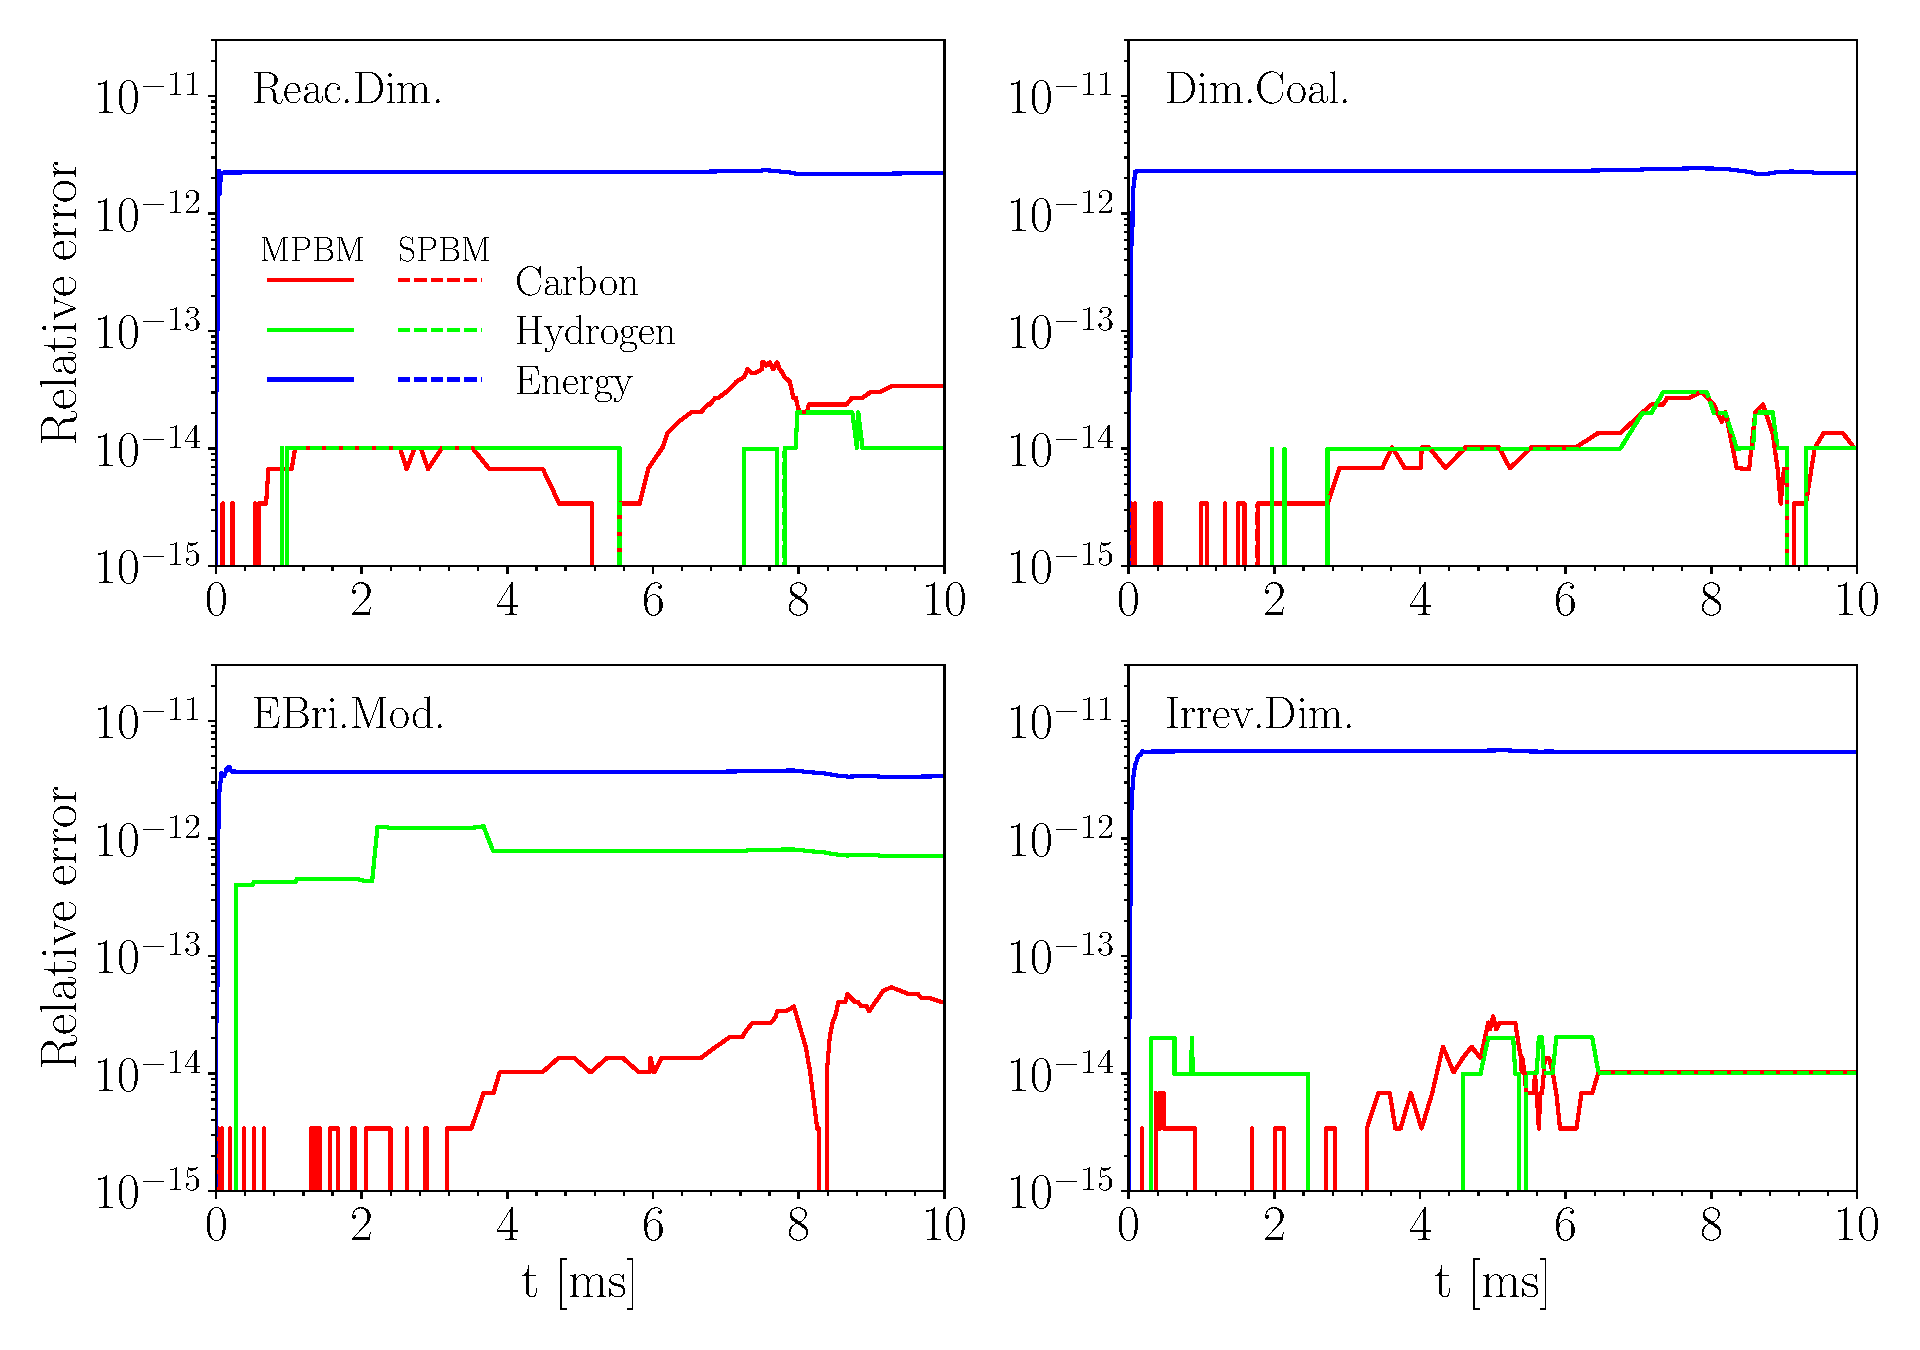
\includegraphics[width=0.8\textwidth]{Figures/Results/Validation/ConstUV/relerr_constuv.pdf}
	\caption{The relative error of total carbon (red line) and hydrogen (green line) mass, and total internal energy residual of gas and soot (blue line) plotted against residence time during pyrolysis of 30\% $\mathrm{CH_4}$-$\mathrm{N_2}$ at 2455 K and 3.47 atm in the constant volume reactor simulated using different PAH growth models along with MPBM (solid line) and SPBM (dashed line).}
	\label{fig:constuvvalid}
\end{figure}


\subsection{Constant Pressure Reactor}
The pyrolysis of 5\% $\mathrm{CH_4}$-Ar in a shock-tube with post-reflected-shock temperature and pressure of 2355 K and 4.64 atm, respectively, was simulated using CPR model. Figure~\ref{fig:cprvalid} shows the relative error of total carbon, hydrogen and energy of system for different PAH growth and particle dynamics models in the constant pressure that falls below $\mathrm{10^{-10}}$ for all parameters confirming the validity of model in satisfying the mass and energy balance in the constant pressure reactor using all models.

\begin{figure}[H]
	\centering
	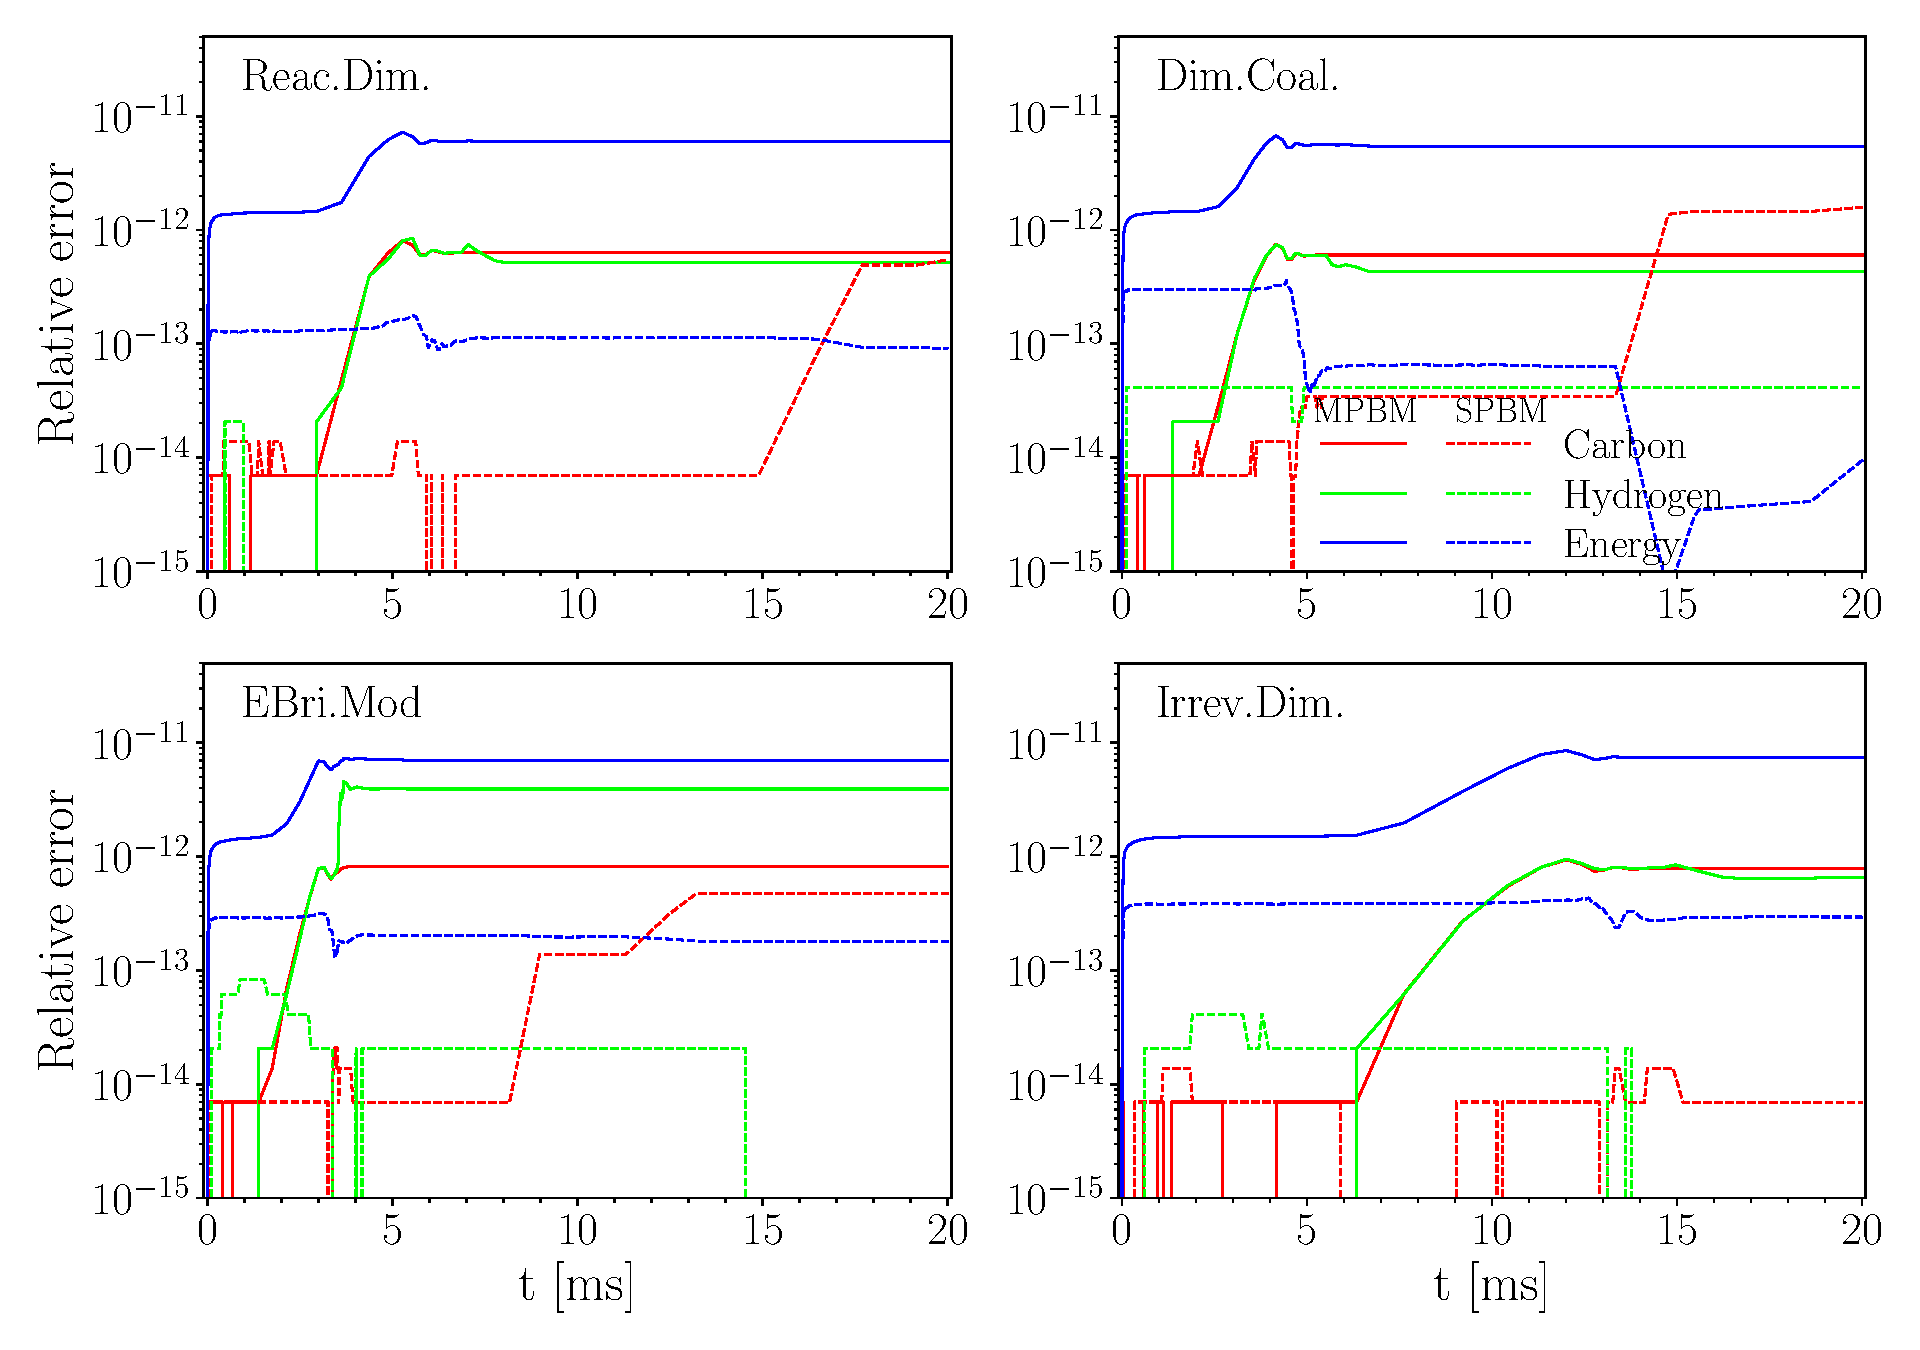
\includegraphics[width=0.8\textwidth]{Figures/Results/Validation/CPR/relerr_cpr.pdf}
	\caption{The relative error of total carbon (red line) and hydrogen (green line) mass, and total internal energy residual of gas and soot (blue line) plotted against residence time during pyrolysis of 5\% $\mathrm{CH_4}$-Ar at 2355 K and 4.64 atm simulated using CPR with different combinations of PAH growth models and particle dynamics models: MPBM (solid line) and SPBM (dashed line).}
	\label{fig:cprvalid}
\end{figure}

\subsection{Perfectly Stirred Reactor}
\label{sec:psrvalid}
The mass and energy balance are investigated for soot formation during ethylene-air oxidation at equivalence ratio of $\phi=2$ in a perfectly stirred reactor. The simulation conditions were chosen based on the combustor implemented and utilized by \citet{stouffer2002combustion}. The reactants enter the reactor with the volume of 250 ml at 300 K and atmospheric pressure. The simulation is initialized from a high temperature ($\approx2000$~K) to avoid trivial solution (cold reactant leaving the reactor with no chemical reactions) and to ensure the model captures a sustained combustion. The residence time of products in the reactor is 8.5 ms. Figure~\ref{fig:psrvalid} shows the relative error of total elemental carbon and hydrogen mass and total enthalpy of gas and soot, which is less than $10^{-6}$ for all combinations of particle dynamics and PAH growth models.

\begin{figure}[H]
	\centering
	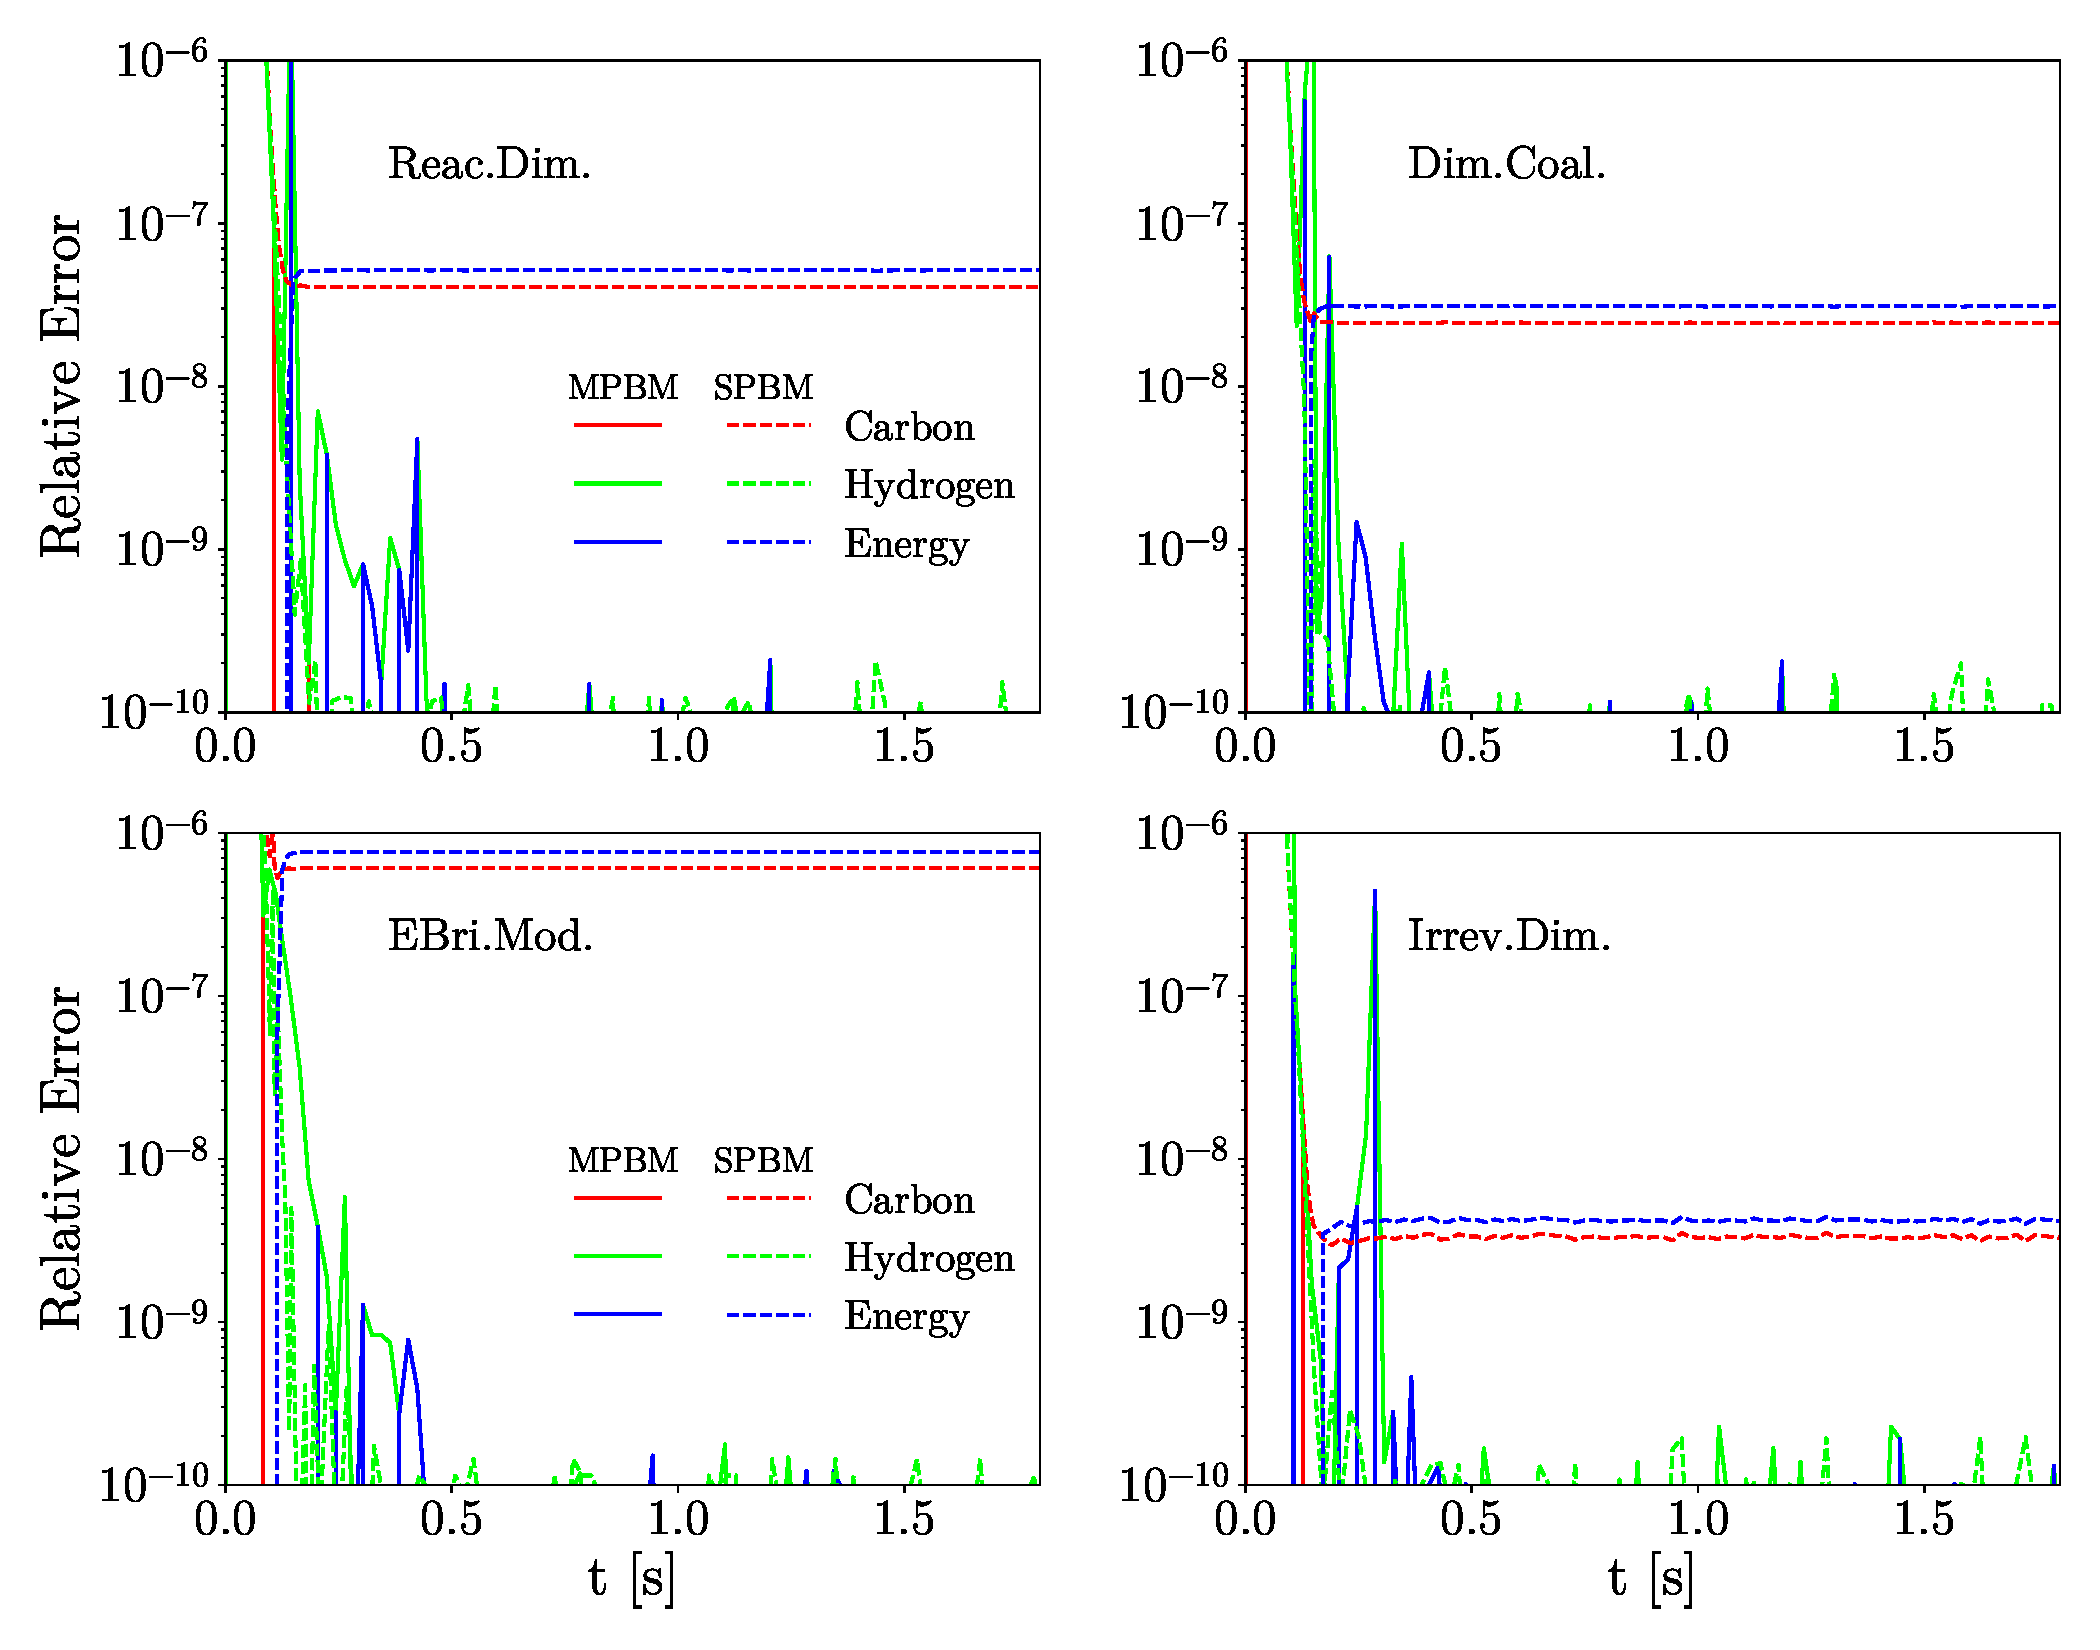
\includegraphics[width=0.8\textwidth]{Figures/Results/Validation/PSR/relerr_psr.pdf}
	\caption{The relative error of total carbon (red line) and hydrogen (green line) mass, and total internal energy residual of gas and soot (blue line) plotted in simulation time during adiabatic combustion of $\mathrm{C_2H_4}$-air with $\phi=2$ at 1 atm simulated using different combinations of PAH growth models and particle dynamics models: MPBM (solid line) and SPBM (dashed line).}
	\label{fig:psrvalid}
\end{figure}


\subsection{Plug Flow Reactor}
Methane pyrolysis in an adiabatic PFR was used to assess the conservation of elemental carbon, hydrogen, and energy. The inlet stream 30\% $\mathrm{CH_4}$ diluted in $\mathrm{N_2}$ with an initial temperature of 2100 K and pressure of 1 atm. Figure~\ref{fig:pfrvalid} shows the residuals of total elemental carbon, hydrogen, and energy along the reactor length, up to 40 cm, for all combinations of PAH growth and particle dynamics models. The residuals remain below $10^{-11}$, confirming that the PFR model in Omnisoot satisfies mass and energy conservation.

\begin{figure}[H]
	\centering
	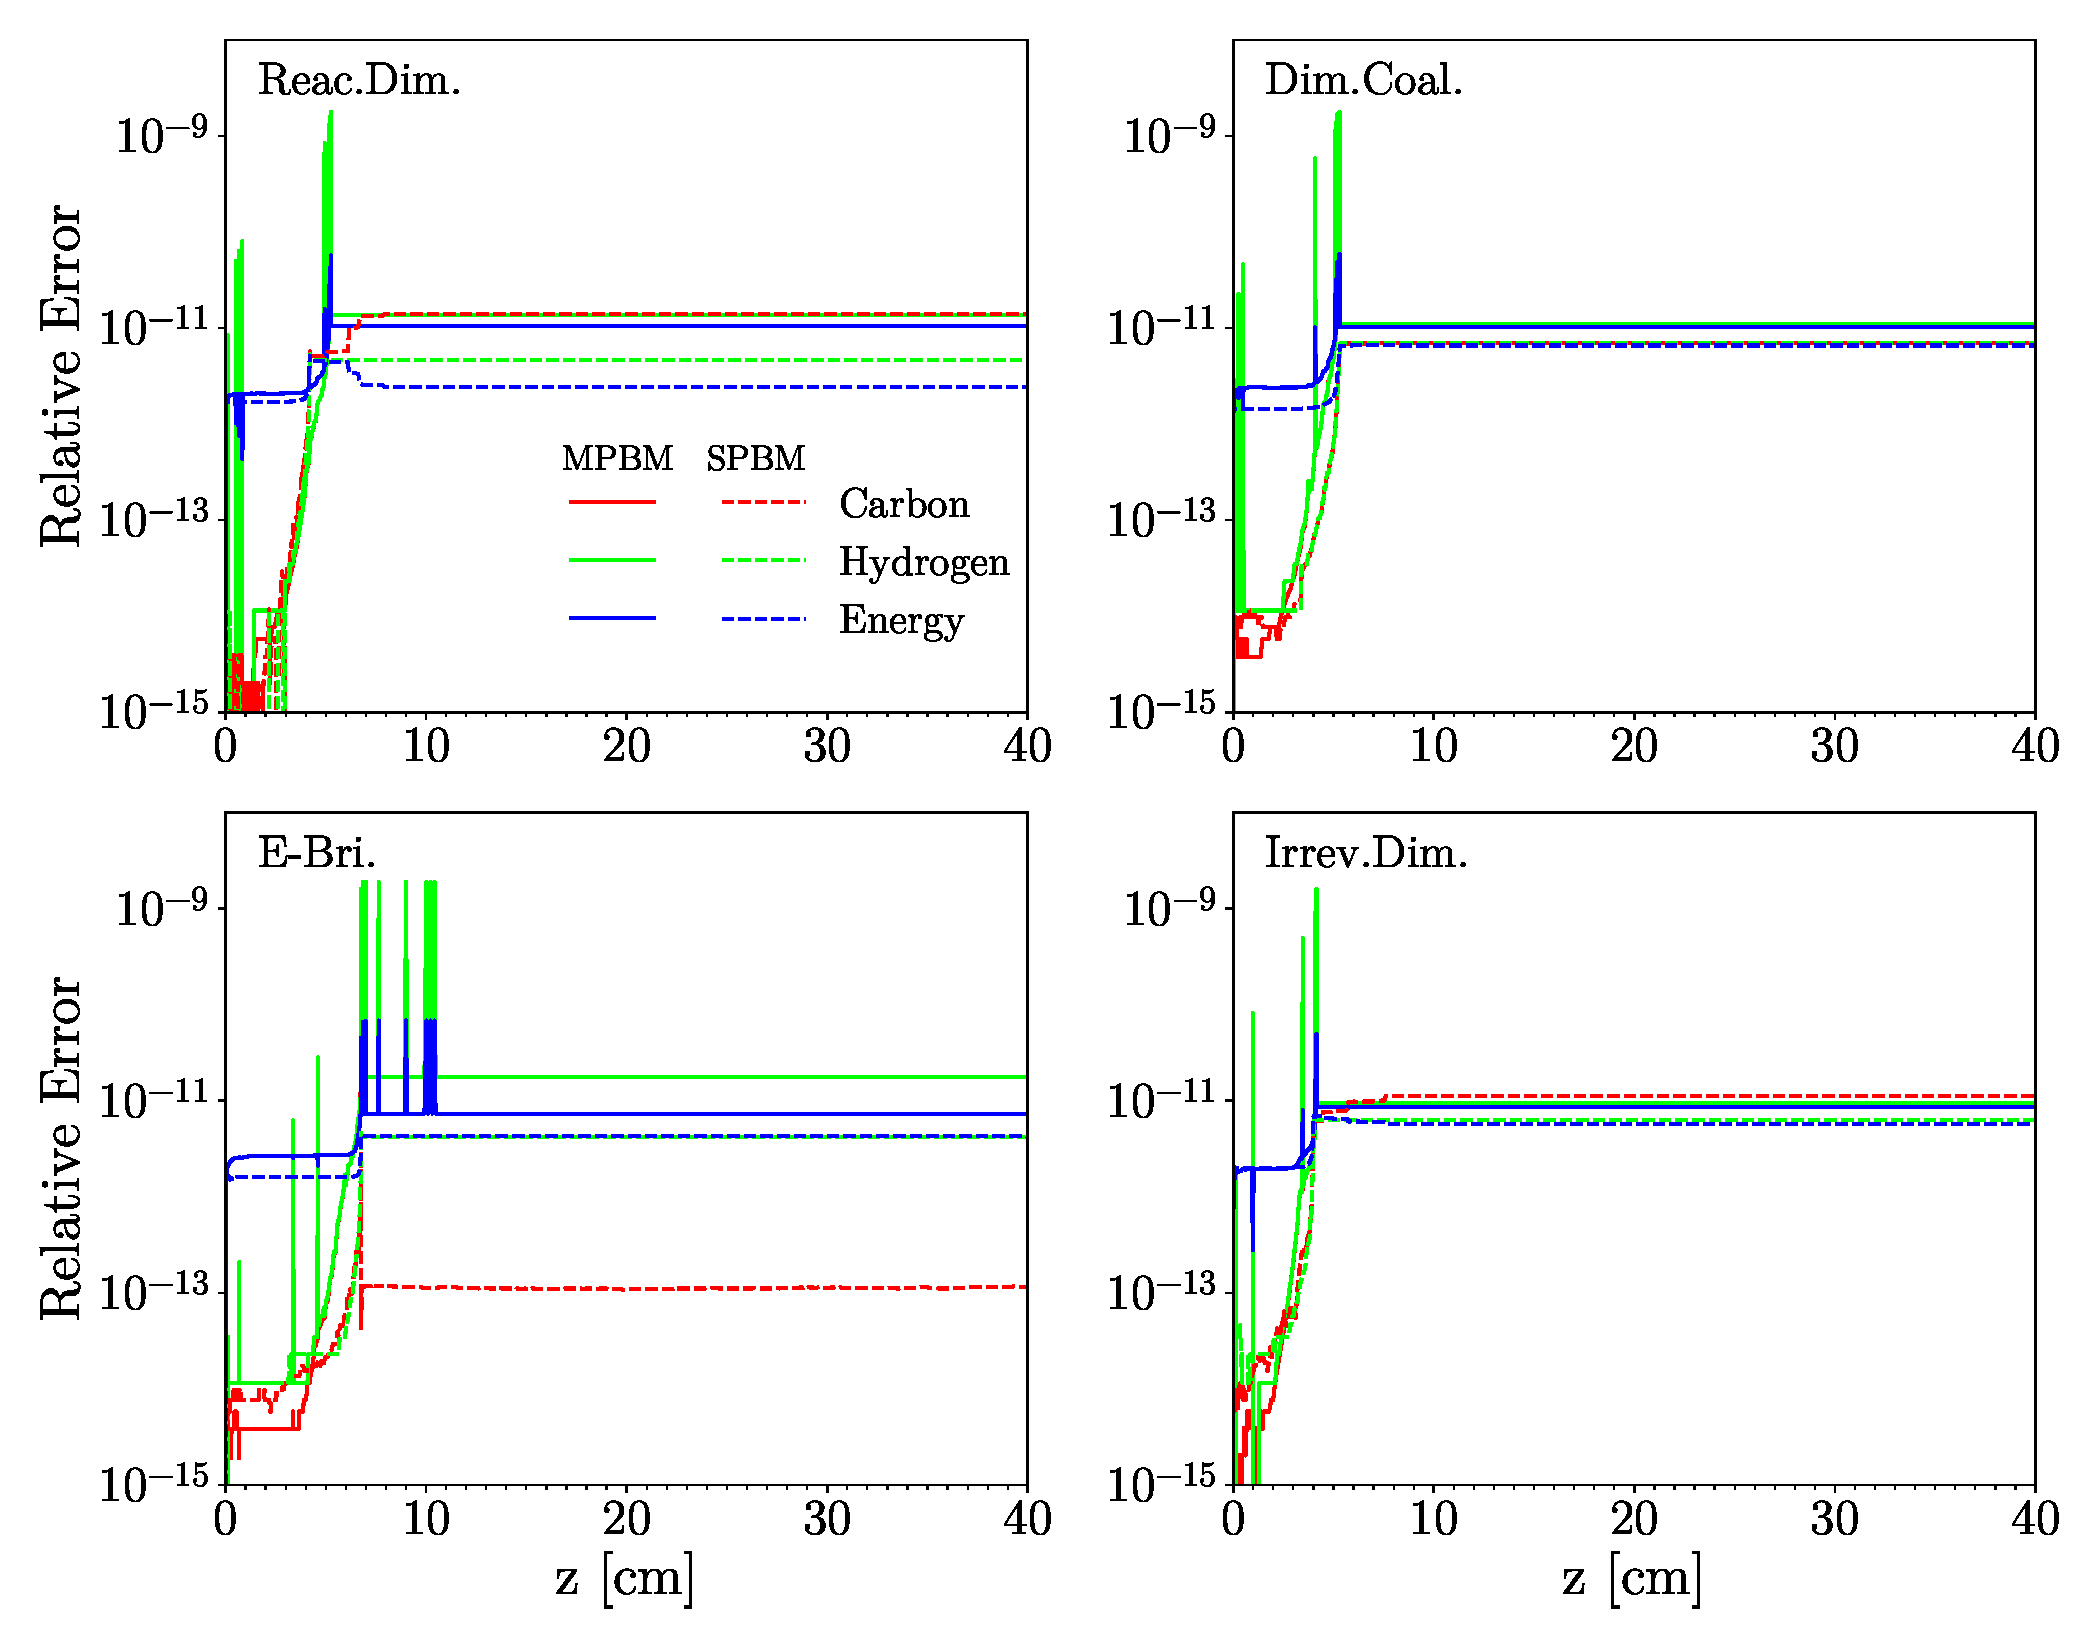
\includegraphics[width=0.8\textwidth]{Figures/Results/Validation/PFR/relerr_pfr.pdf}
	\caption{The relative error of total carbon (red line), hydrogen (green line) mass, and total internal energy residual of gas and soot (blue line) plotted against reactor length (cm) in the adiabatic flow reactor during pyrolysis of 30\%~$\mathrm{CH_4}$-$\mathrm{N_2}$ at 2100 K and 1 atm simulated using different combinations of PAH growth models and particle dynamics models: MPBM (solid line) and SPBM (dashed line).}
	\label{fig:pfrvalid}
\end{figure}


\section{Validation of Collision Frequency}
\label{sec:validcolfreq}
The collision frequency function determines the rate at which two particles collide, which results in the reduction of the total number of agglomerates and the increase in particle size. In the absence of strong flow shear or external forces, Brownian motion is the main driving force for particle coagulation. As explained in Sections~\ref{sec:sectextra} and \ref{sec:mpbm}, Omnisoot employs harmonic mean and Fuchs interpolations to calculate collision frequency of agglomerates from free-molecular ($\mathrm{Kn}\ge10$) to continuum ($\mathrm{Kn}\le0.1$) regimes based on the gas mean free path and the particle size. 


The test case for validation of collision frequency is based on the DEM simulation of 2000 monodisperse spherical particles with the density of 2200 $\mathrm{kg/m^3}$ in
a cubic cell with the constant temperature of 298 K and pressure of 1 atm~\citep{goudeli2015coagulation}. Figure~\ref{fig:kernelvalid} depicts the collision frequency plotted against Knudsen number ($\mathrm{Kn}=2\lambda/d_m$) obtained by Omnisoot using harmonic mean (red solid line) and Fuchs interpolation (blue dashed line) and DEM results of \citet{goudeli2015coagulation}. The Fuchs interpretation perfectly matches DEM data over the free-molecular regime to the continuum regime. Harmonic mean is also in good agreement with the DEM results in the free-molecular and continuum regimes, but slightly underpredicts the collision frequency in the transition regime with relative errors less than 16\%.

\begin{figure}[H]
	\centering
	\begin{tikzpicture}
		\draw (0, 0) node[inner sep=0] 	{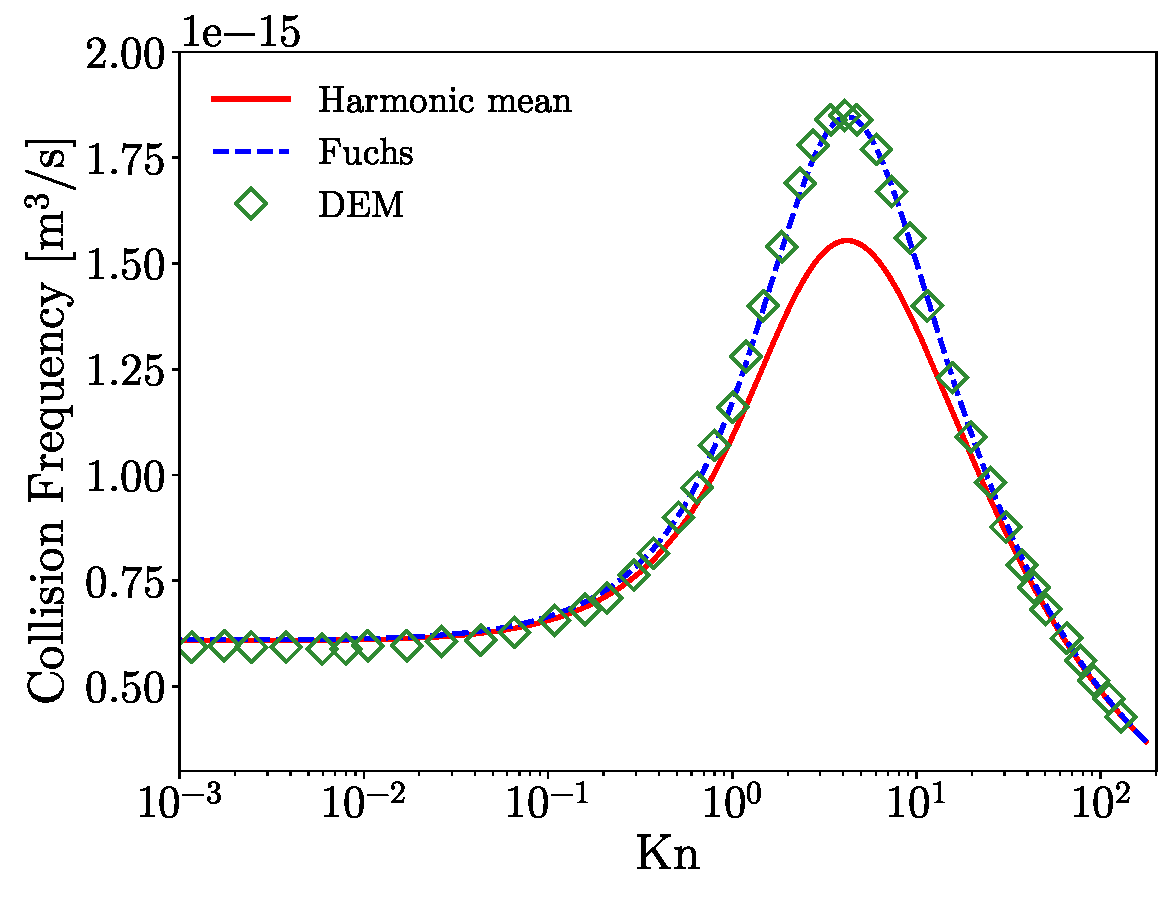
\includegraphics[width=0.45\textwidth]{Figures/Results/Validation/Kernel/kernel_valid.pdf}};
		\draw (-0.33, 1.11) node {\footnotesize{\cite{goudeli2015coagulation}}};
	\end{tikzpicture}
	\caption{The comparison of collision frequency, $\beta$, obtained by Omnisoot using harmonic mean (red solid line) and Fuchs interpolations (blue dashed line) with DEM results (symbols)~\citep{goudeli2015coagulation}.}
	\label{fig:kernelvalid} 
\end{figure}


%\section{The comparison of A2, A2R5, and A4 predicted using different reaction mechanisms}
%
%\begin{figure}[H]
%	\centering
%	\begin{subfigure}[t]{0.32\textwidth}
%		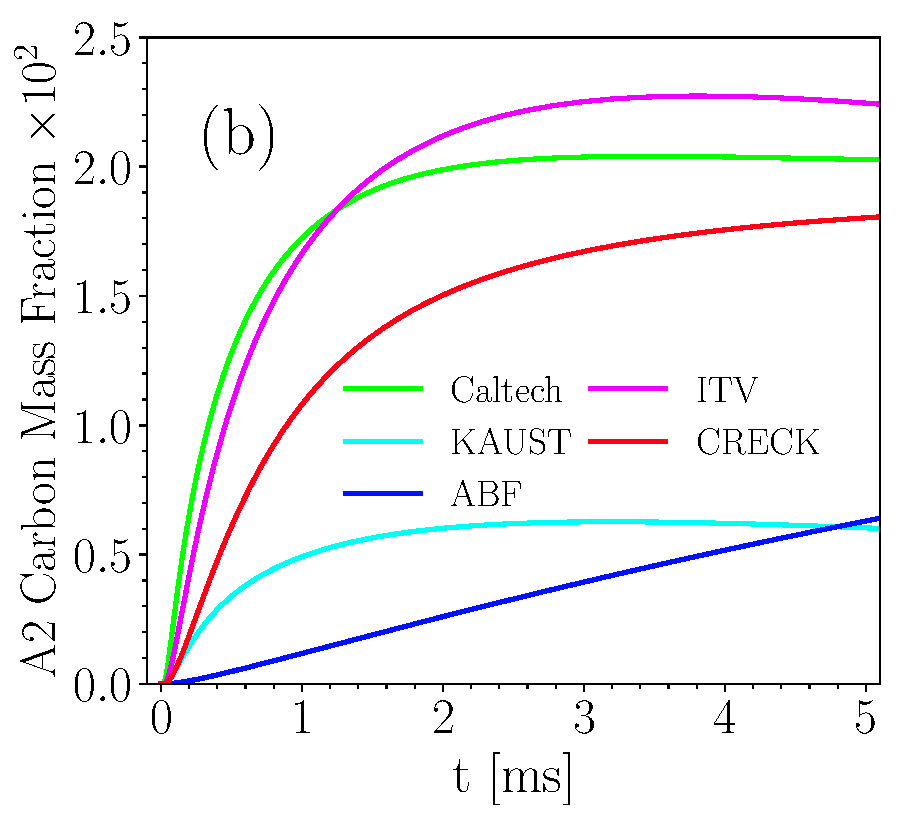
\includegraphics[width=1\textwidth]{Figures/Results/chemistry/A2.pdf}
%	\end{subfigure}
%	\begin{subfigure}[t]{0.32\textwidth}
%		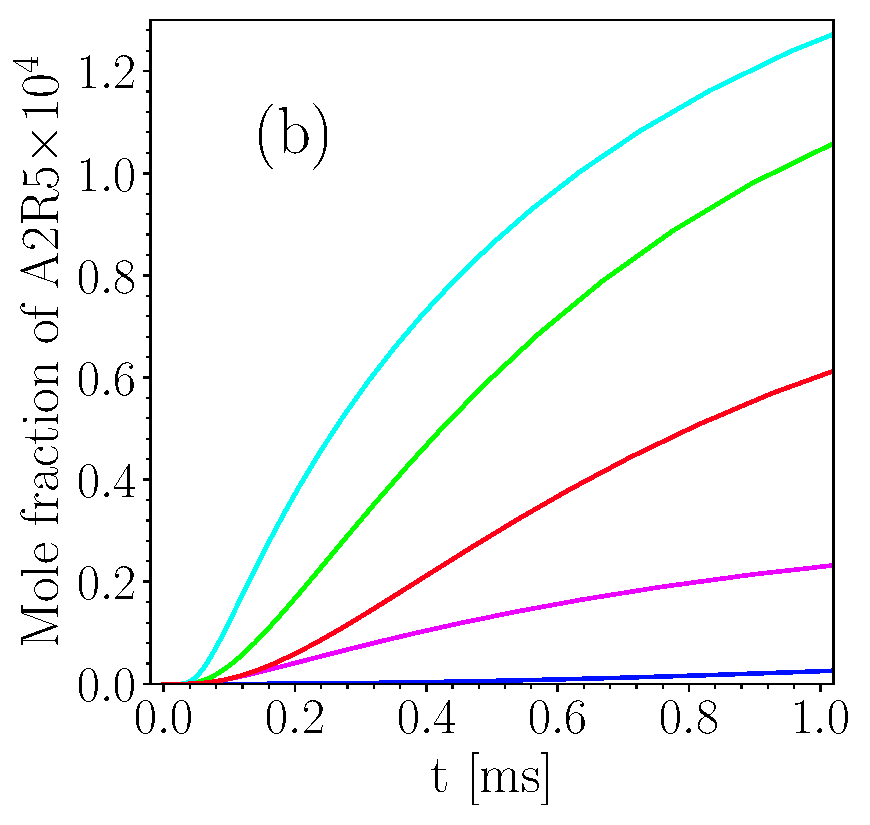
\includegraphics[width=1\textwidth]{Figures/Results/chemistry/A2R5.pdf}
%	\end{subfigure}
%	\begin{subfigure}[t]{0.32\textwidth}
%		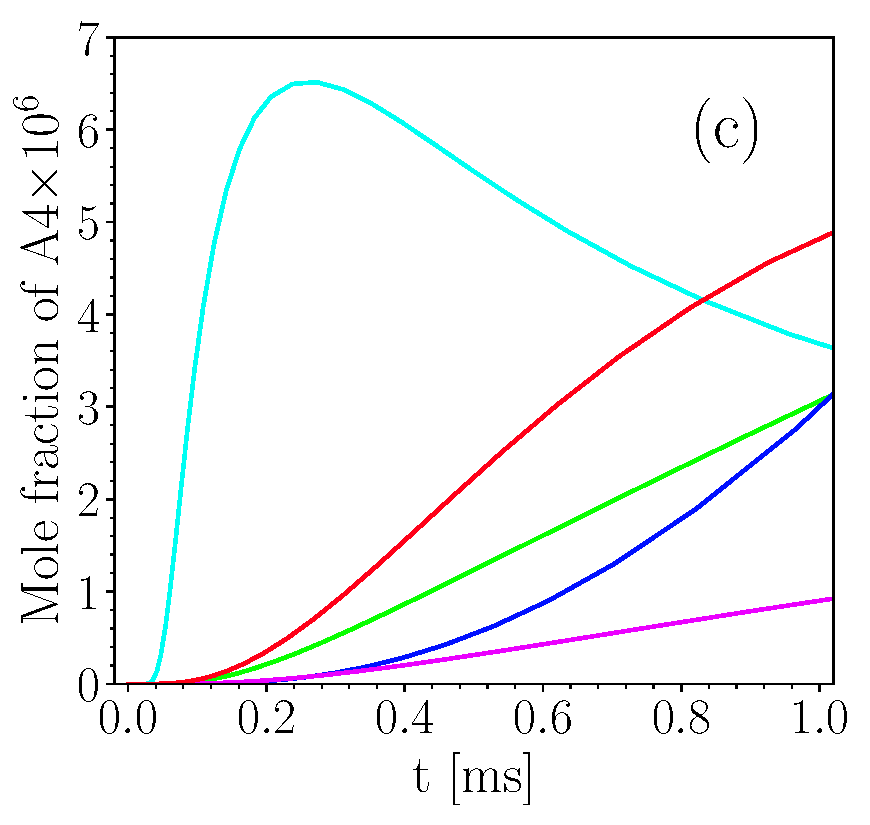
\includegraphics[width=1\textwidth]{Figures/Results/chemistry/A4.pdf}
%	\end{subfigure}
%	\caption{The mole fraction of A2 (a), A2R5 (b), and A4 (c) during pyrolysis of 5\%~$\mathrm{CH_4}$-Ar predicted using different reaction mechanism.}
%	\label{fig:AAA_chem} 
%\end{figure}

\section{The comparison of maximum possible soot volume fraction predicted using different reaction mechanisms}

\begin{figure}[H]
	\centering
	\begin{tikzpicture}
		\draw (0, 0) node[inner sep=0] 	{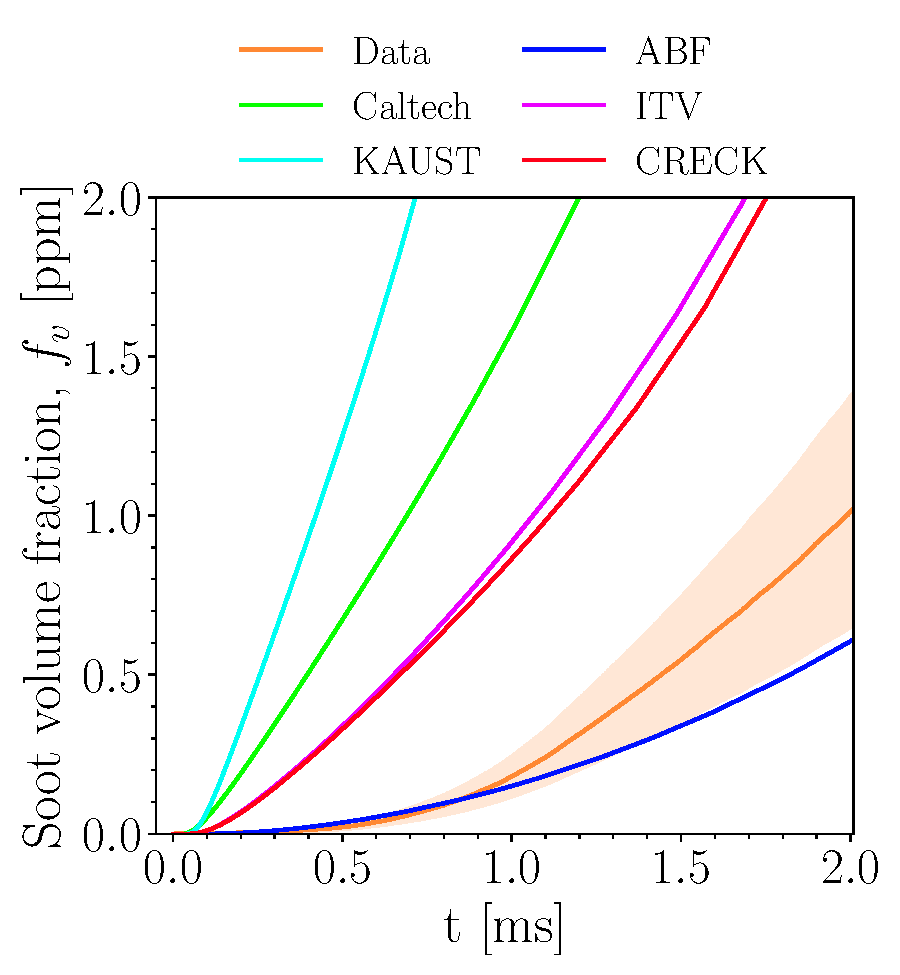
\includegraphics[width=0.35\textwidth]{Figures/Results/chemistry/soot_fv_max.pdf}};
		\draw (0.11, 2.58) node {\tiny{\hl{[G]}}};
	\end{tikzpicture}
	\caption{The maximum soot volume fraction predicted using Irreversible Dimerization and different reaction mechanisms during pyrolysis of 5\%~$\mathrm{CH_4}$-Ar was compared with measurements~[\hl{GB}]. The shaded area represents the uncertainty in the reported experimental data.}
	\label{fig:max_sootfv_chem} 
\end{figure}

\section{The comparison of Monodisperse and Sectional population balance models}

\begin{figure}[H]
	\centering
	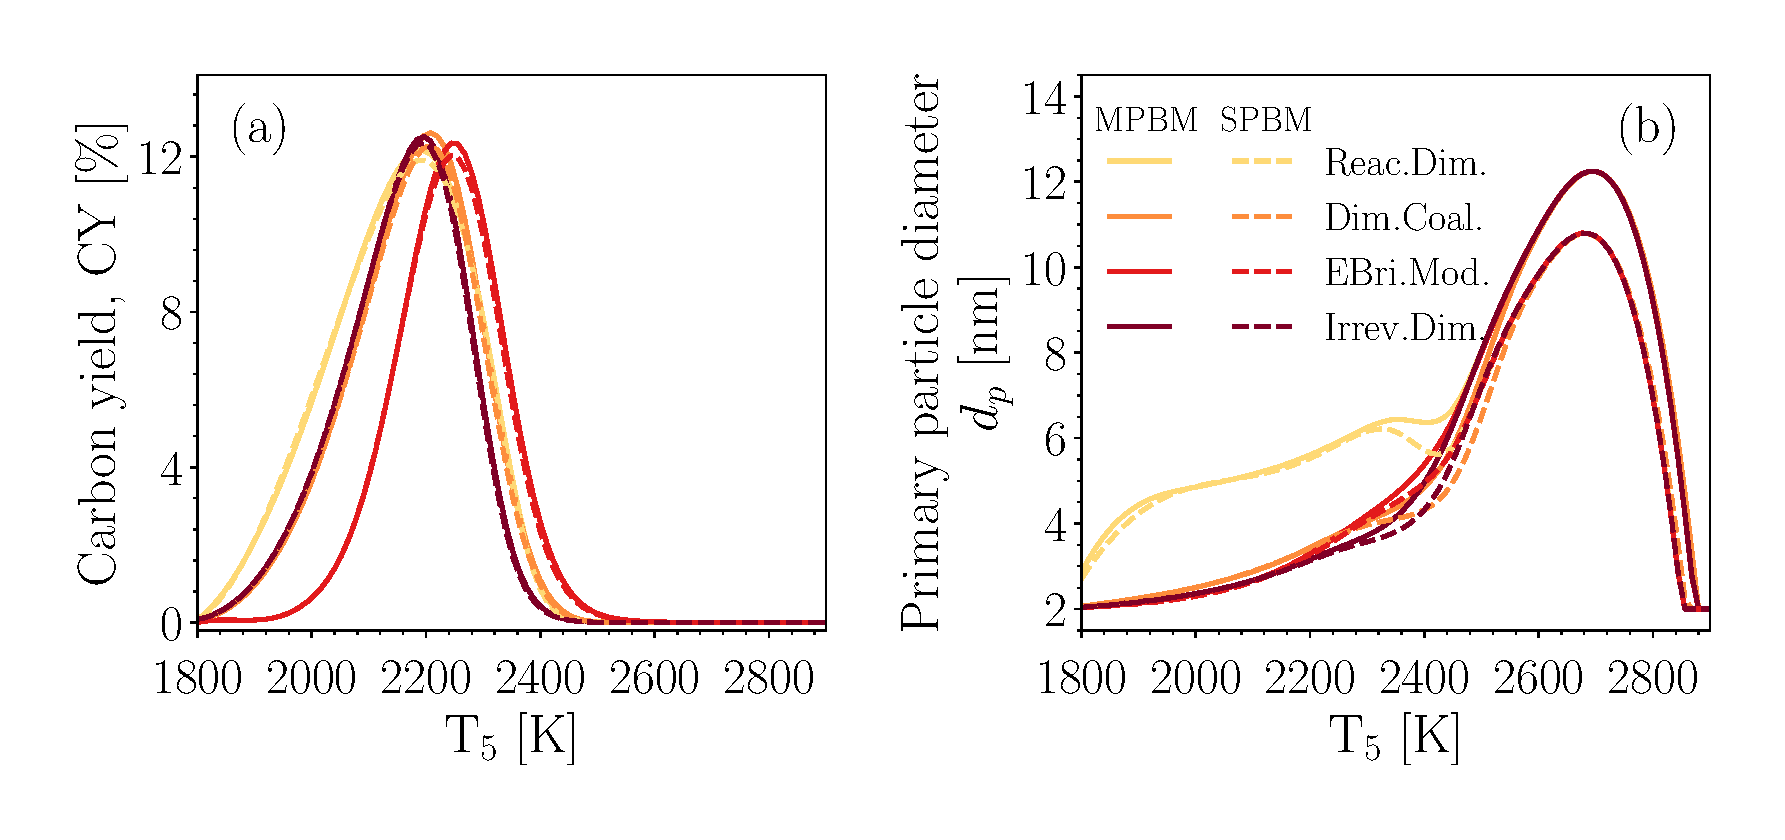
\includegraphics[width=0.8\textwidth]{Figures/Results/Shocktube/Agafonov2016_cpr/carbon_yield_d_p_pdynamics.pdf};
	\caption{The comparison of CY (a) and primary particle diameter, $d_p$, at $t=$1.5 ms obtained using MPBM and SPBM models for the case optimized using equal adjustment factors to minimize the prediction error.}
	\label{fig:shockagof_yield_dp_cpr_pdynamics} 
\end{figure}


\begin{figure}[H]
	\centering
	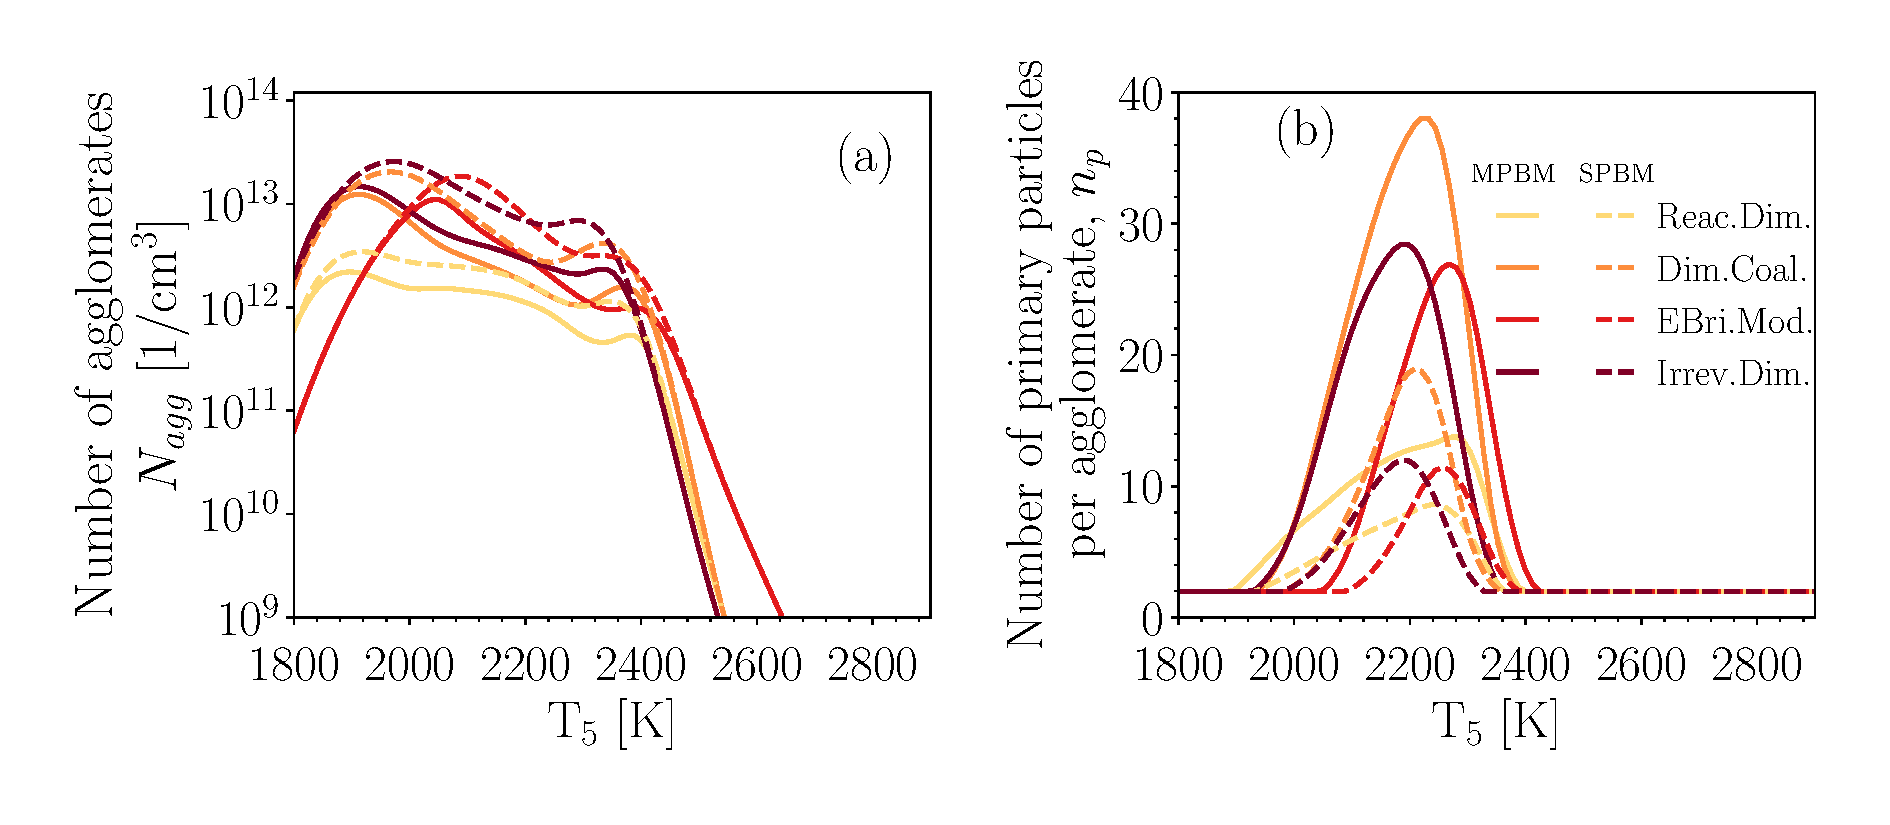
\includegraphics[width=0.8\textwidth]{Figures/Results/Shocktube/Agafonov2016_cpr/N_agg_n_p_pdynamics.pdf};
	\caption{The temperature dependence of total number of agglomerates, $N_{agg}$ (a), number of primary particles per agglomerate, $n_p$ (b), at $t=$1.5 ms obtained using MPBM and SPBM models for the case optimized using equal adjustment factors to minimize the prediction error.}
	\label{fig:shockagof_N_agg_n_p_cpr_pdynamics} 
\end{figure}

\begin{figure}[H]
	\centering
	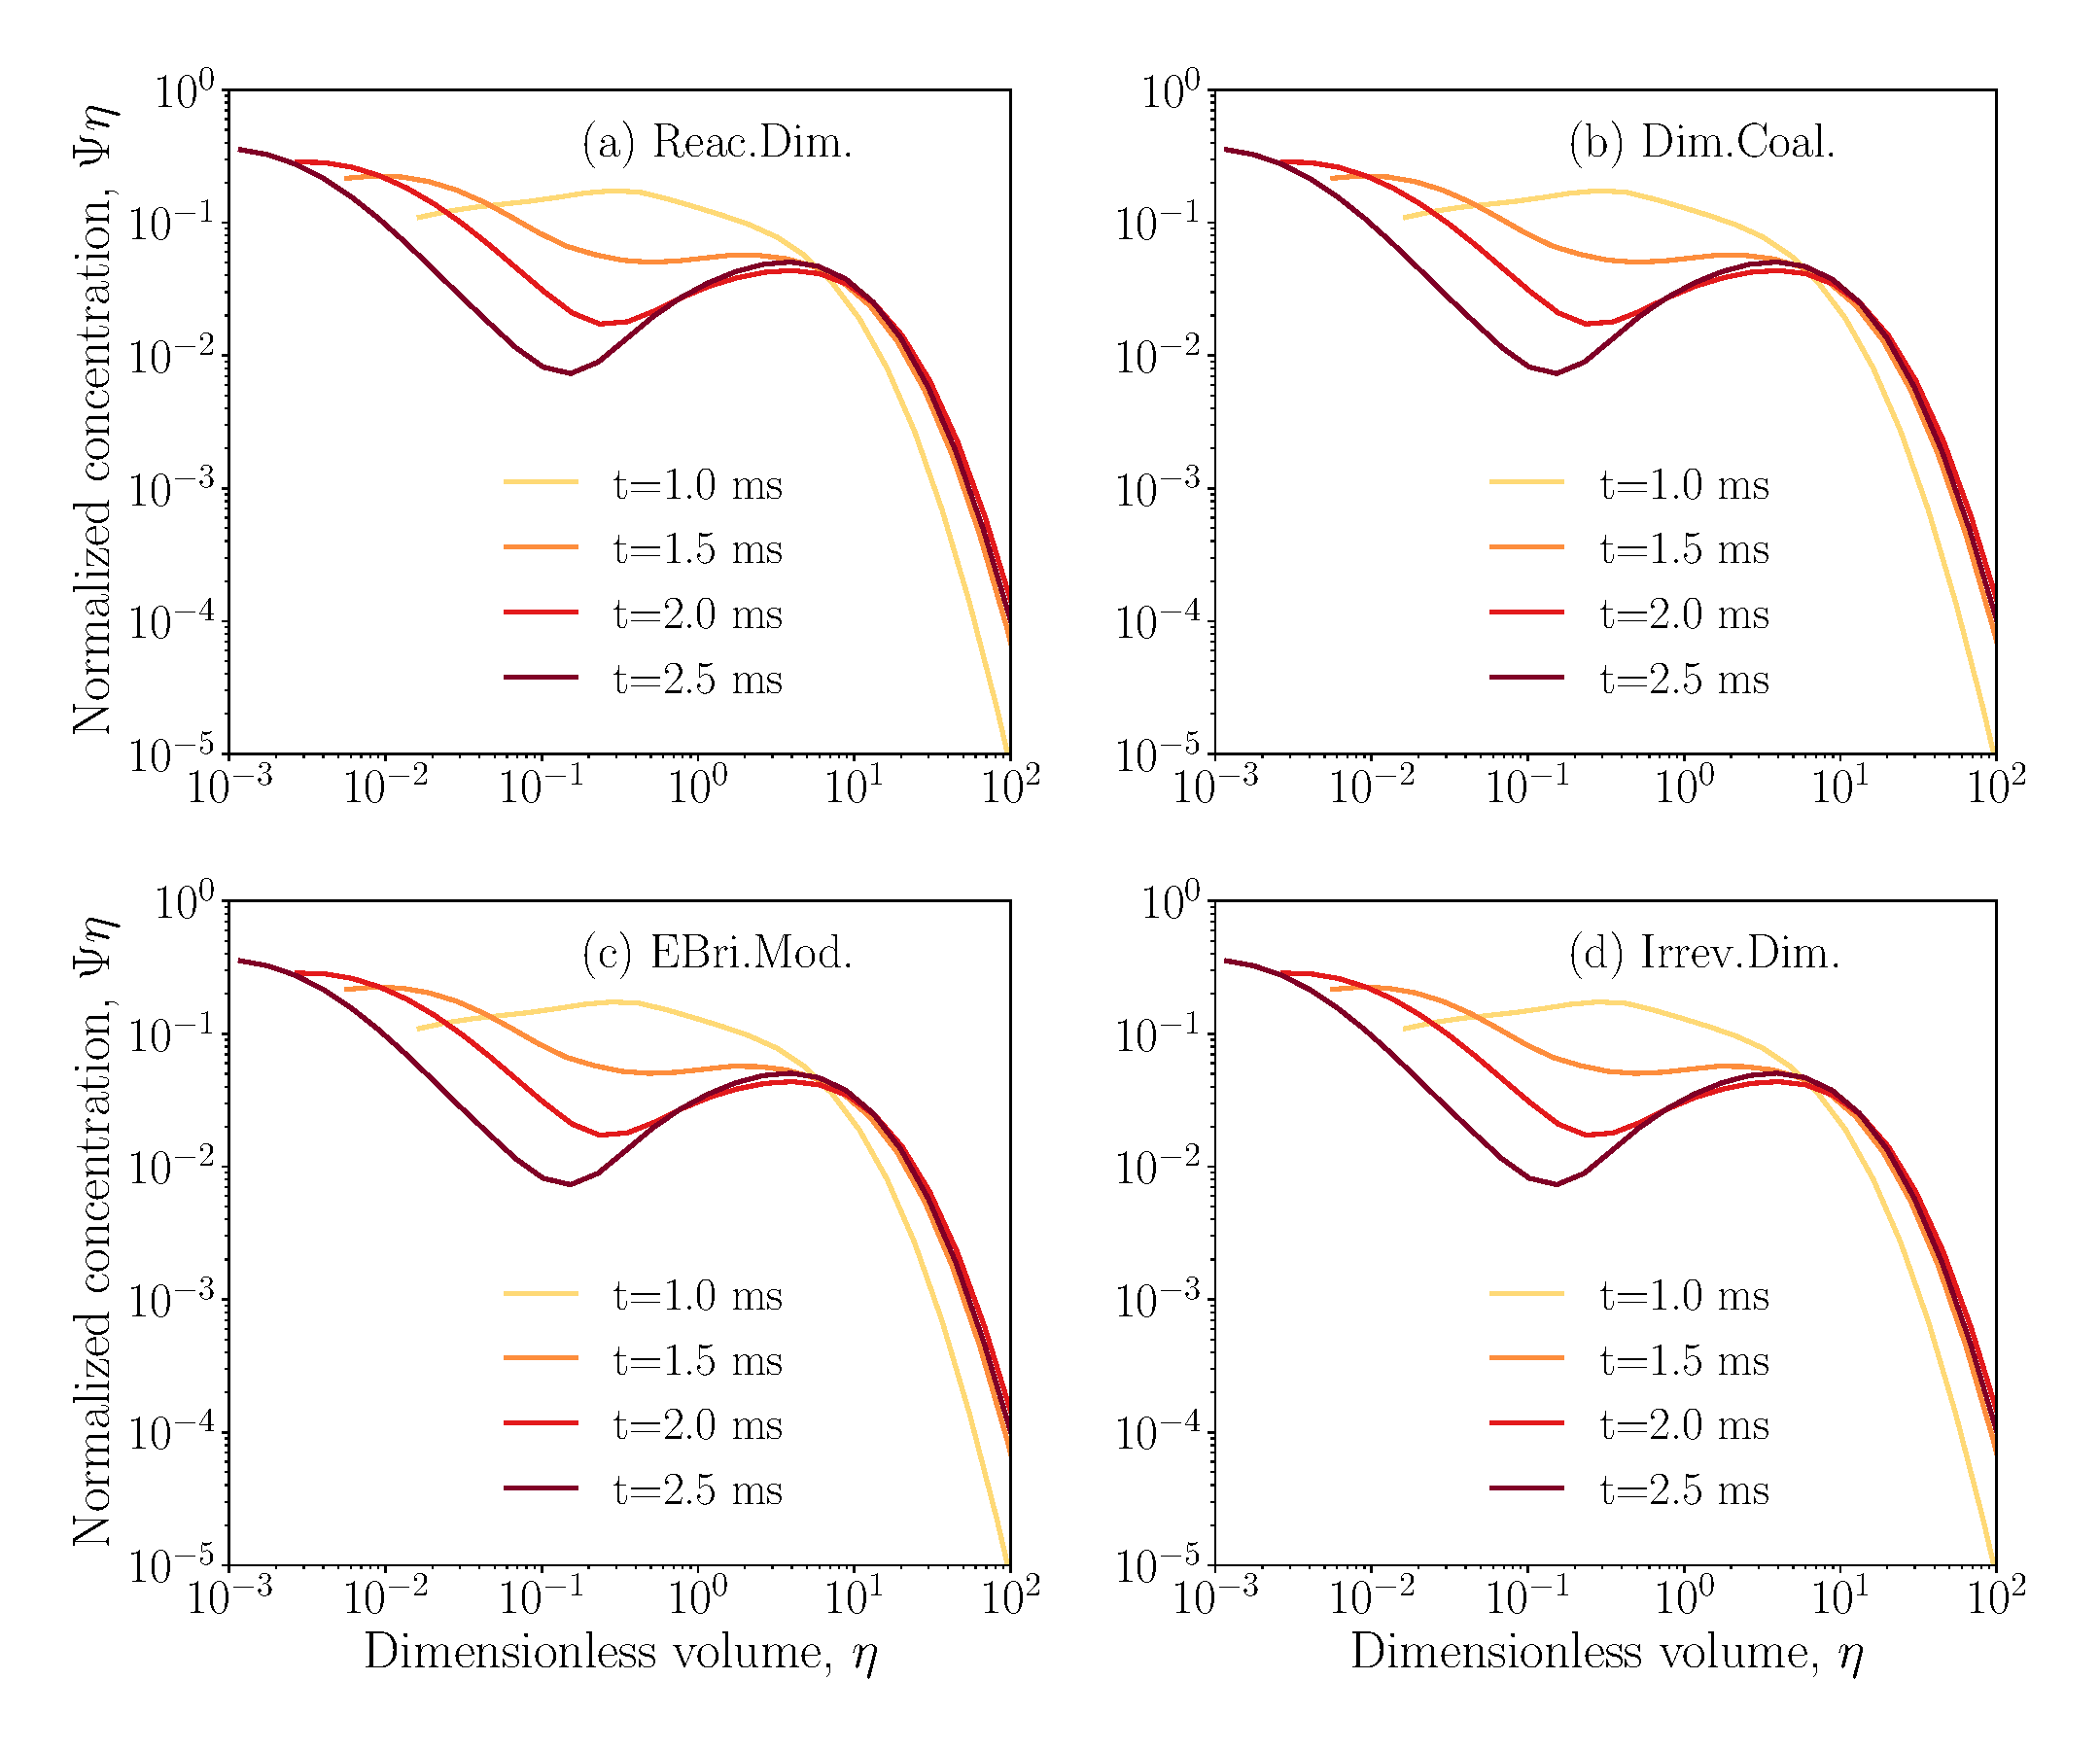
\includegraphics[width=0.8\textwidth]{Figures/Results/Shocktube/Agafonov2016_cpr/5CH4_psd.pdf};
	\caption{The non-dimensional particle size distribution during 5\%$\mathrm{CH_4}$-Ar at $\mathrm{T_5}=2200$ K that evolves from 1~ms to 2.5~ms indicating SPSD is not attained yet.}
	\label{fig:shockagof_psd} 
\end{figure}

\section{The Effect of Excluding Five-membered Rings}

\begin{figure}[H]
	\centering
	\begin{tikzpicture}
		\draw (0, 0) node[inner sep=0] 	{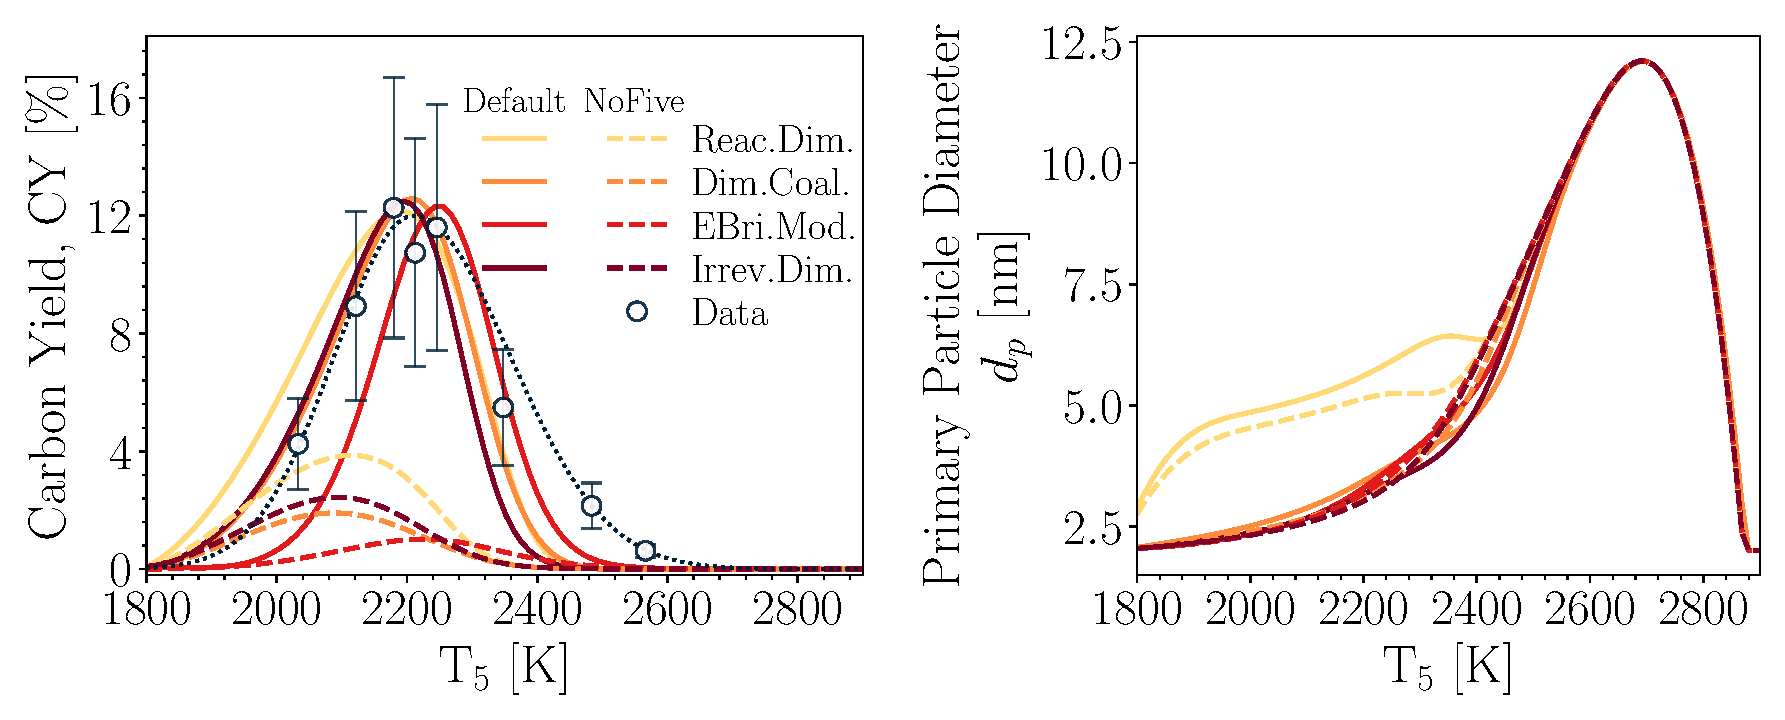
\includegraphics[width=0.8\textwidth]{Figures/Results/Shocktube/Agafonov2016_cpr/carbon_yield_dp_spc_combined.pdf}};
		\draw (-0.55, 0.29) node {\scriptsize{\cite{agafonov2016unified}}};
		%\draw (2.42, -0.23) node {\scriptsize{\cite{agafonov2016unified}}};
	\end{tikzpicture}
	\caption{The soot carbon yield, CY, at $t=$1.5 ms (a) and primary particle diameter, $d_p$ (b) obtained using the default soot precursors listed in Table~\ref{tab:precursors_list} (denoted by solid line and labeled as ``Default") compared with the same results when five-membered ring PAHs  excluded from soot precursors (denoted by dashed line and labeled as ``NoFive"). Both cases were obtained using Caltech mechanism and the same equal adjustment factors. The black dashed line was added to show the trend in the measurements~\citep{agafonov2016unified}.}
	\label{fig:shockagof_yieldspc_cpr} 
\end{figure}

\begin{figure}[H]
	\centering
	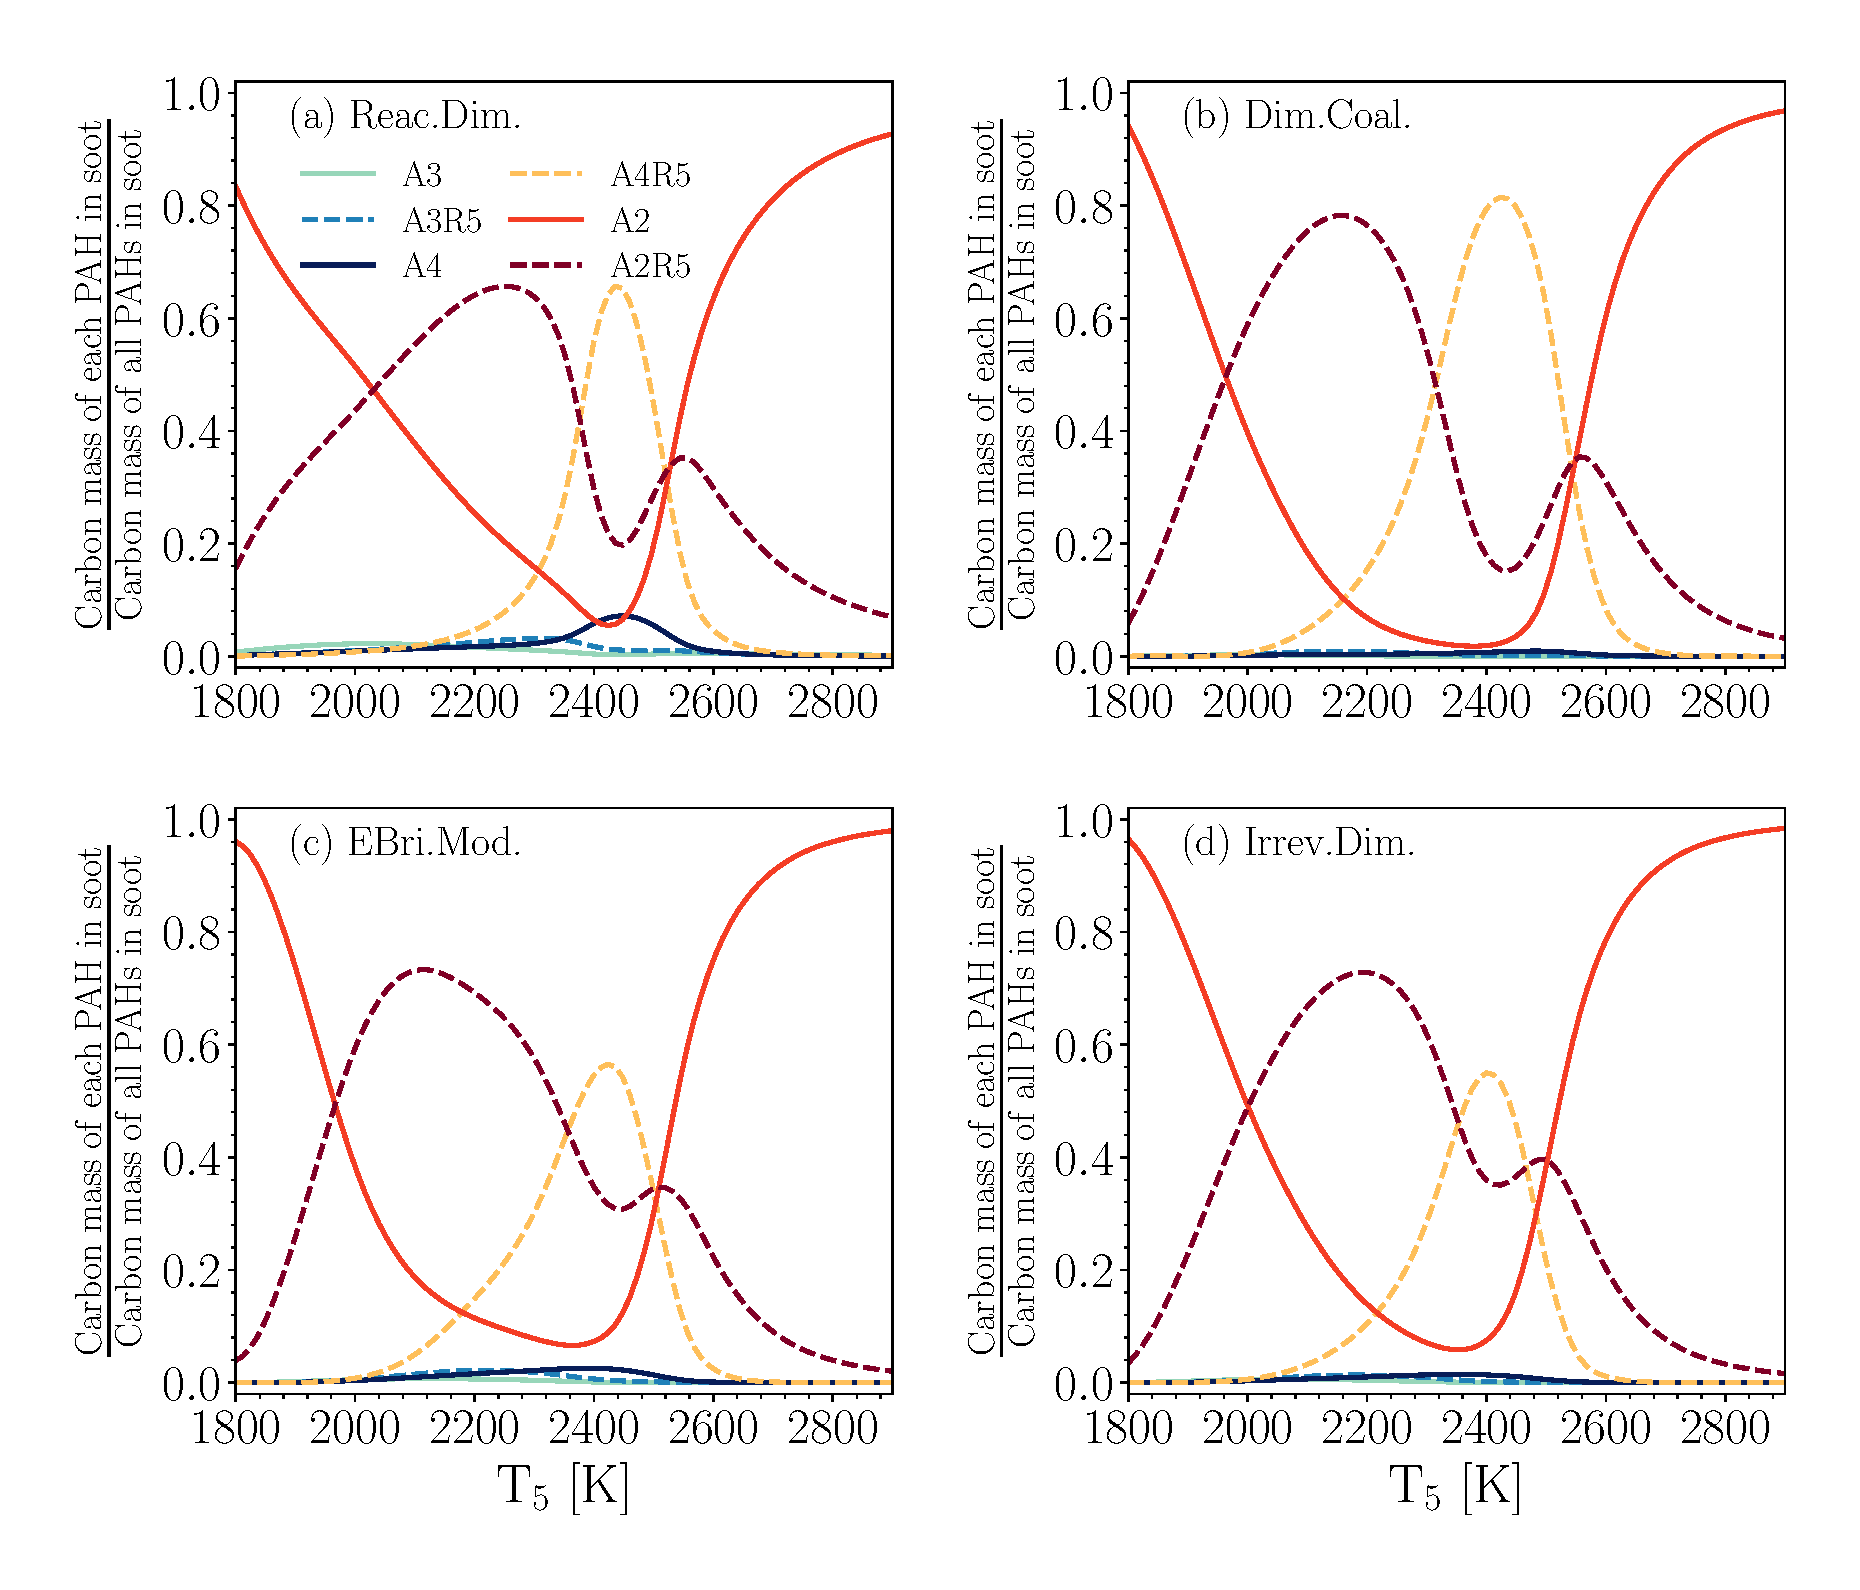
\includegraphics[width=0.8\textwidth]{Figures/Results/Shocktube/Agafonov2016_cpr/c_dist_spc.pdf}
	\caption{The contribution of each soot precursor to total carbon mass from precursors, at $t=$1.5 ms obtained using Caltech mechanisms, SPBM, and different inception models during 5\%$\mathrm{CH_4}$-Ar pyrolysis.}
	\label{fig:shockagof_spccont_cpr} 
\end{figure}

\section{Ethylene pyrolysis in a flow reactor}


\begin{figure}[H]
	\centering
	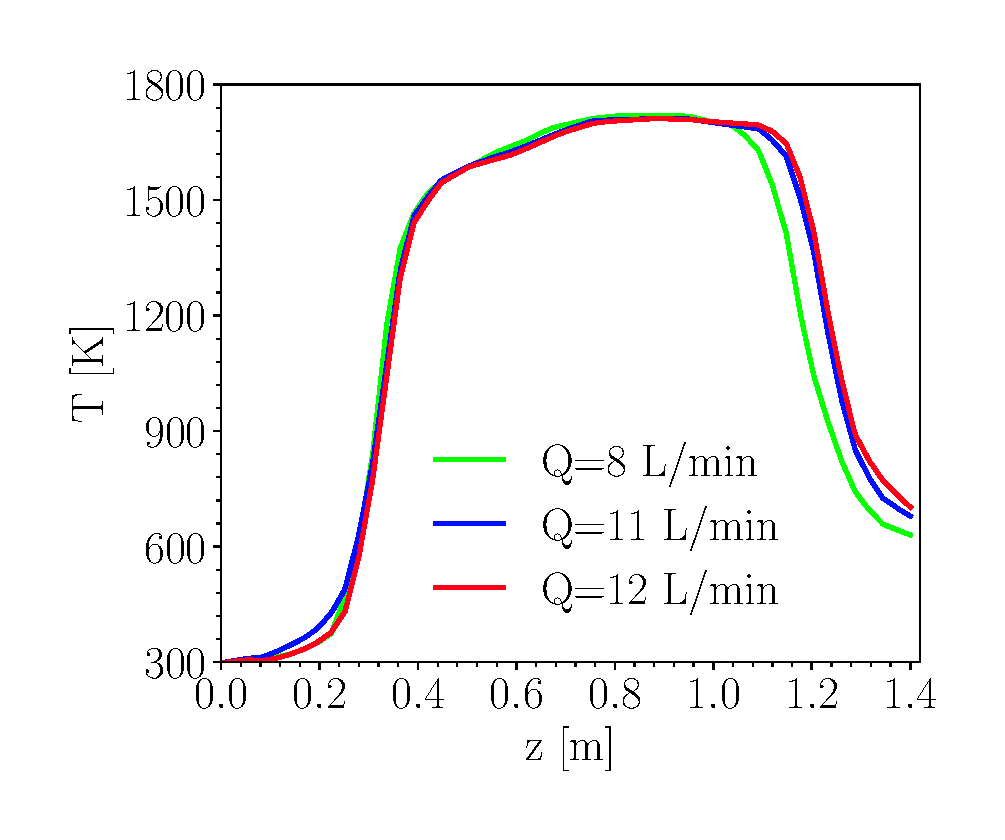
\includegraphics[width=0.45\textwidth]{Figures/Results/PFR/temperature_combined.pdf}
	\caption{The centerline temperature along the reactor for $\mathrm{Q}=8$, 11, and 12 L/min interpolated from the thermocouple measurements~\citep{mei2019quantitative}.}
	\label{fig:pfr_temp} 
\end{figure}


\begin{figure}[H]
	\centering
	\begin{tikzpicture}
		\draw (0, 0) node[inner sep=0] 	{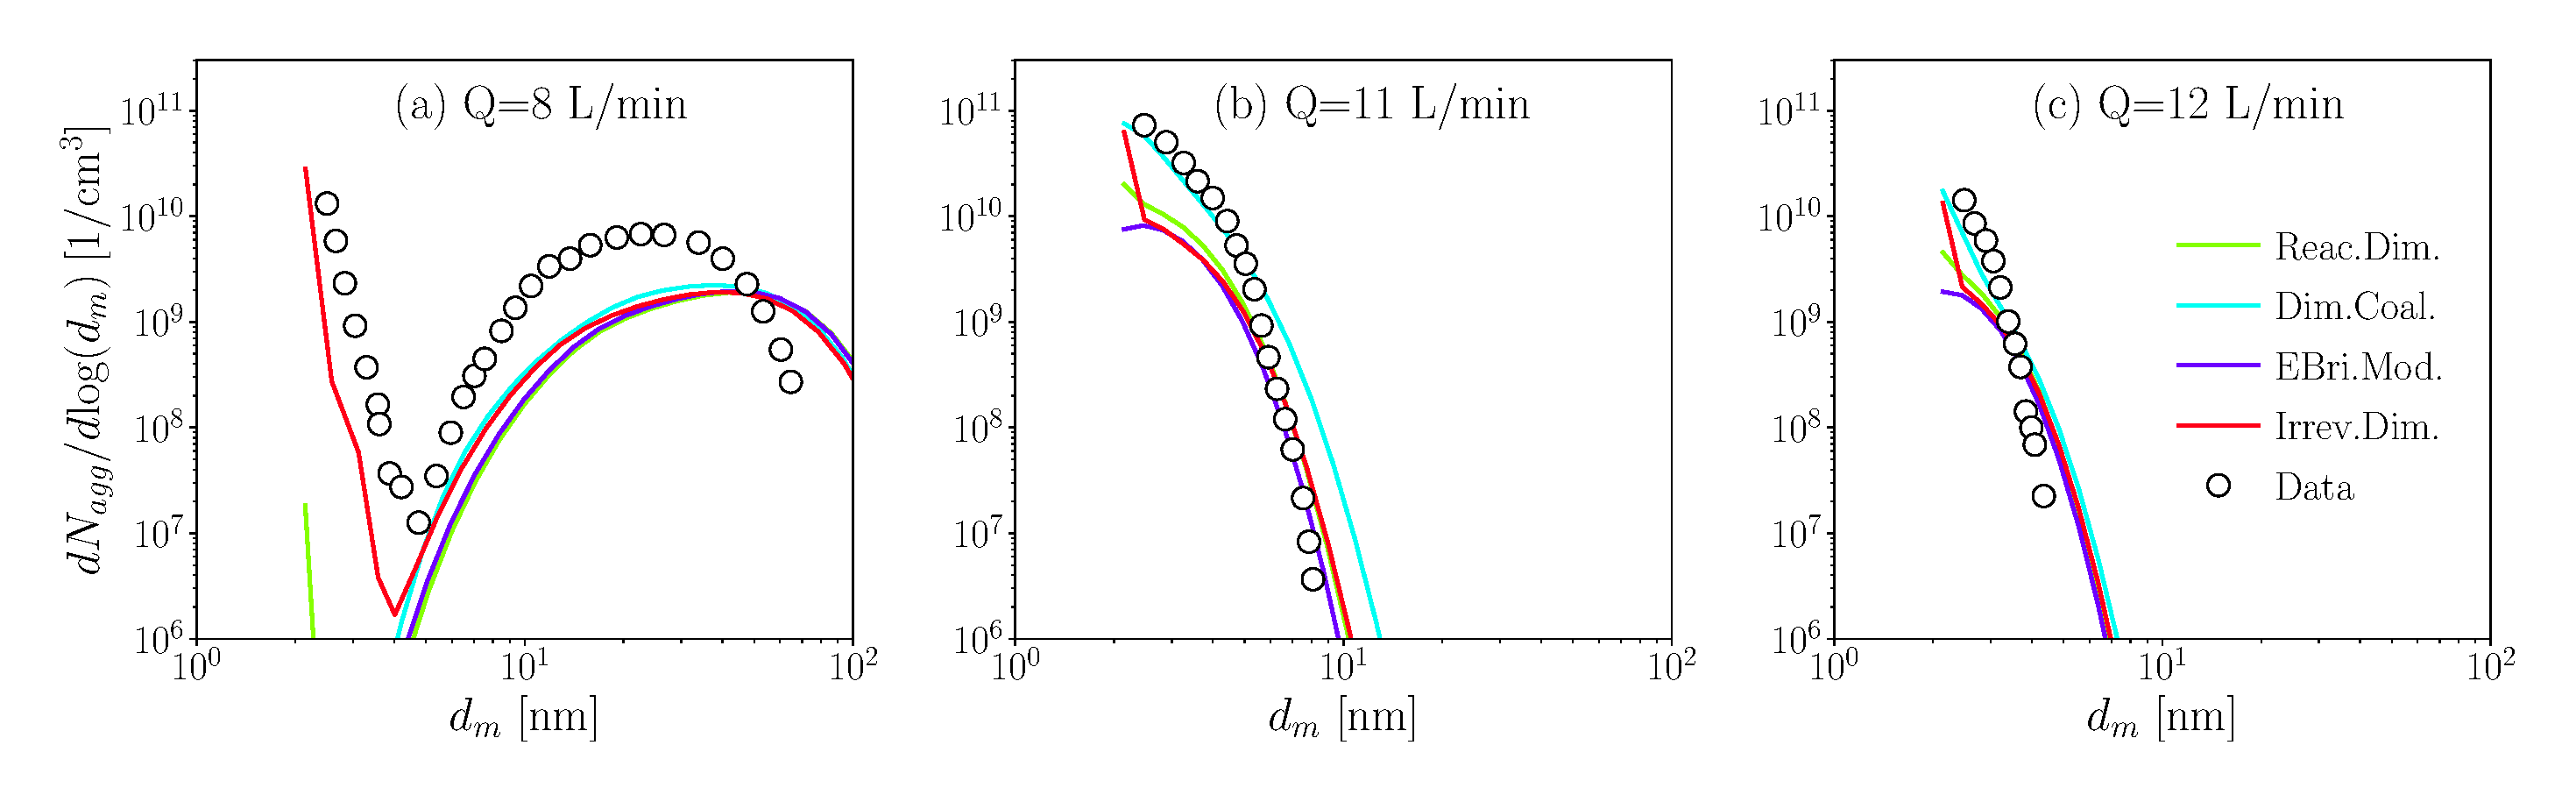
\includegraphics[width=1\textwidth]{Figures/Results/PFR/PSD_diffQ_caltech.pdf}};
		\draw (6.63, -0.51) node {\scriptsize{\cite{mei2019quantitative}}};
	\end{tikzpicture}
	\caption{The particle size distribution at the end of PFR for $\mathrm{Q}=8$ (a), 11 (b), and 12 L/min (c) obtained using Caltech mechanism, SPBM and different inception models calibrated to match the predictions with measurement~\citep{mei2019quantitative}.}
	\label{fig:pfr_psd_caltech} 
\end{figure}


\begin{figure}[H]
	\centering
	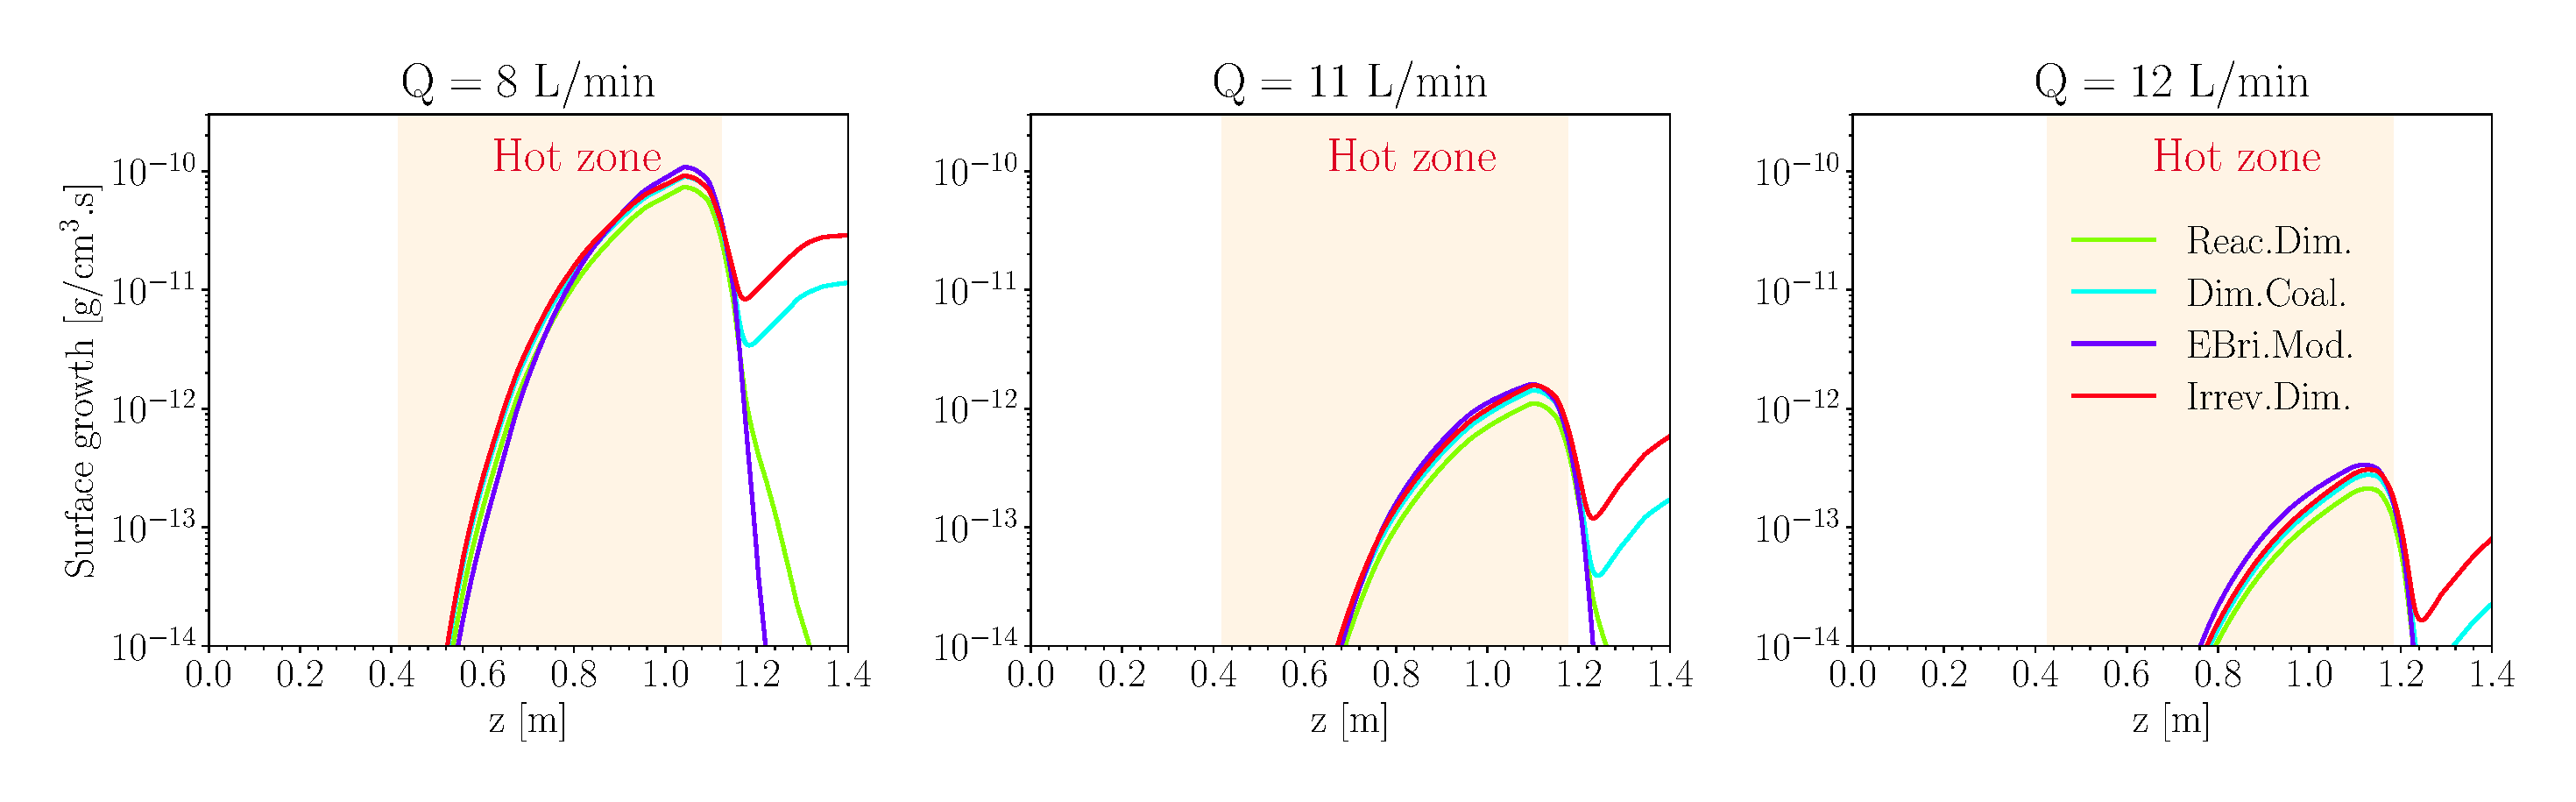
\includegraphics[width=1\textwidth]{Figures/Results/PFR/surface_growth.pdf}
	\caption{The surface growth by HACA and PAH adsorption combined along the PFR for $\mathrm{Q}=8$ (a), 11 (b), and 12 L/min (c) obtained using KAUST mechanism, SPBM and different inception models. The yellow area represents the hot zone ($\mathrm{T}>0.9\mathrm{T_{max}}$).}
	\label{fig:pfr_surfacegrowth} 
\end{figure}



\section{Ethylene oxidation in a perfectly stirred reactor}

\begin{table}[H]
	\centering
	\caption{The geometric mean mobility diameter, $d_{m,g}$, and the geometric mobility standard deviation, $\sigma_{m,g}$, obtained using different inception models compared with the value calculated from the measured PSD~\citep{manzello2007soot}.}
	\label{tab:psrpfr_morpcomp}
	%\begin{tabular}{l|ll|ll|ll|}
	\begin{tabular}{lllllll}
		\cline{2-7}
		& \multicolumn{2}{c}{$\phi=1.9$}                   & \multicolumn{2}{c}{$\phi=2.0$} & \multicolumn{2}{c}{$\phi=2.1$} \\ \cline{2-7} 
		& \multicolumn{1}{l} {$d_{m,g}$  [nm]} & $\sigma_{m,g}$ & \multicolumn{1}{l} {$d_{m,g}$  [nm]} &  $\sigma_{m,g}$ & \multicolumn{1}{l}{$d_{m,g}$  [nm]} & $\sigma_{m,g}$ \\ \hline
		\multicolumn{1}{l}{\textbf{Data}~\citep{manzello2007soot}}                      & \multicolumn{1}{l}{\textbf{6.04}}          &     \textbf{1.25}      & \multicolumn{1}{l}{\textbf{12.40}} &  \textbf{1.49} & \multicolumn{1}{l}{\textbf{17.66}} & \textbf{1.64} \\ %\hline
		\multicolumn{1}{l}{Reactive Dimerization}     & \multicolumn{1}{l}{8.27}          &    1.14       & \multicolumn{1}{l}{11.10} & 1.21  & \multicolumn{1}{l}{16.88} & 1.58  \\ %\hline
		\multicolumn{1}{l}{Dimer Coalescence}         & \multicolumn{1}{l}{8.18}          &      1.14     & \multicolumn{1}{l}{10.76} & 1.24 & \multicolumn{1}{l}{16.99} & 1.68 \\ %\hline
		\multicolumn{1}{l}{E-Bridge Modified}          & \multicolumn{1}{l}{8.27}          &    1.15       & \multicolumn{1}{l}{11.02} & 1.27 & \multicolumn{1}{l}{14.56} & 1.58 \\ %\hline
		\multicolumn{1}{l}{Irreversible Dimerization} & \multicolumn{1}{l}{8.19}          &      1.14     & \multicolumn{1}{l}{10.96} & 1.25 & \multicolumn{1}{l}{18.44} & 1.78 \\ \hline
	\end{tabular}
\end{table}
